
%% bare_jrnl.tex
%% V1.4a
%% 2014/09/17
%% by Michael Shell
%% see http://www.michaelshell.org/
%% for current contact information.
%%
%% This is a skeleton file demonstrating the use of IEEEtran.cls
%% (requires IEEEtran.cls version 1.8a or later) with an IEEE
%% journal paper.
%%
%% Support sites:
%% http://www.michaelshell.org/tex/ieeetran/
%% http://www.ctan.org/tex-archive/macros/latex/contrib/IEEEtran/
%% and
%% http://www.ieee.org/

%%*************************************************************************
%% Legal Notice:
%% This code is offered as-is without any warranty either expressed or
%% implied; without even the implied warranty of MERCHANTABILITY or
%% FITNESS FOR A PARTICULAR PURPOSE! 
%% User assumes all risk.
%% In no event shall IEEE or any contributor to this code be liable for
%% any damages or losses, including, but not limited to, incidental,
%% consequential, or any other damages, resulting from the use or misuse
%% of any information contained here.
%%
%% All comments are the opinions of their respective authors and are not
%% necessarily endorsed by the IEEE.
%%
%% This work is distributed under the LaTeX Project Public License (LPPL)
%% ( http://www.latex-project.org/ ) version 1.3, and may be freely used,
%% distributed and modified. A copy of the LPPL, version 1.3, is included
%% in the base LaTeX documentation of all distributions of LaTeX released
%% 2003/12/01 or later.
%% Retain all contribution notices and credits.
%% ** Modified files should be clearly indicated as such, including  **
%% ** renaming them and changing author support contact information. **
%%
%% File list of work: IEEEtran.cls, IEEEtran_HOWTO.pdf, bare_adv.tex,
%%                    bare_conf.tex, bare_jrnl.tex, bare_conf_compsoc.tex,
%%                    bare_jrnl_compsoc.tex, bare_jrnl_transmag.tex
%%*************************************************************************


% *** Authors should verify (and, if needed, correct) their LaTeX system  ***
% *** with the testflow diagnostic prior to trusting their LaTeX platform ***
% *** with production work. IEEE's font choices and paper sizes can       ***
% *** trigger bugs that do not appear when using other class files.       ***                          ***
% The testflow support page is at:
% http://www.michaelshell.org/tex/testflow/



\documentclass[journal]{IEEEtran}
%
% If IEEEtran.cls has not been installed into the LaTeX system files,
% manually specify the path to it like:
% \documentclass[journal]{../sty/IEEEtran}





% Some very useful LaTeX packages include:
% (uncomment the ones you want to load)


% *** MISC UTILITY PACKAGES ***
%
%\usepackage{ifpdf}
% Heiko Oberdiek's ifpdf.sty is very useful if you need conditional
% compilation based on whether the output is pdf or dvi.
% usage:
% \ifpdf
%   % pdf code
% \else
%   % dvi code
% \fi
% The latest version of ifpdf.sty can be obtained from:
% http://www.ctan.org/tex-archive/macros/latex/contrib/oberdiek/
% Also, note that IEEEtran.cls V1.7 and later provides a builtin
% \ifCLASSINFOpdf conditional that works the same way.
% When switching from latex to pdflatex and vice-versa, the compiler may
% have to be run twice to clear warning/error messages.






% *** CITATION PACKAGES ***
%
\usepackage[noadjust]{cite}
% cite.sty was written by Donald Arseneau
% V1.6 and later of IEEEtran pre-defines the format of the cite.sty package
% \cite{} output to follow that of IEEE. Loading the cite package will
% result in citation numbers being automatically sorted and properly
% "compressed/ranged". e.g., [1], [9], [2], [7], [5], [6] without using
% cite.sty will become [1], [2], [5]--[7], [9] using cite.sty. cite.sty's
% \cite will automatically add leading space, if needed. Use cite.sty's
% noadjust option (cite.sty V3.8 and later) if you want to turn this off
% such as if a citation ever needs to be enclosed in parenthesis.
% cite.sty is already installed on most LaTeX systems. Be sure and use
% version 5.0 (2009-03-20) and later if using hyperref.sty.
% The latest version can be obtained at:
% http://www.ctan.org/tex-archive/macros/latex/contrib/cite/
% The documentation is contained in the cite.sty file itself.






% *** GRAPHICS RELATED PACKAGES ***
%
\ifCLASSINFOpdf
  \usepackage[pdftex]{graphicx}
  % declare the path(s) where your graphic files are
  \graphicspath{{../pdf/}{../jpeg/}}
  % and their extensions so you won't have to specify these with
  % every instance of \includegraphics
  \DeclareGraphicsExtensions{.pdf,.jpeg,.png}
\else
  % or other class option (dvipsone, dvipdf, if not using dvips). graphicx
  % will default to the driver specified in the system graphics.cfg if no
  % driver is specified.
  % \usepackage[dvips]{graphicx}
  % declare the path(s) where your graphic files are
  % \graphicspath{{../eps/}}
  % and their extensions so you won't have to specify these with
  % every instance of \includegraphics
  % \DeclareGraphicsExtensions{.eps}
\fi
% graphicx was written by David Carlisle and Sebastian Rahtz. It is
% required if you want graphics, photos, etc. graphicx.sty is already
% installed on most LaTeX systems. The latest version and documentation
% can be obtained at: 
% http://www.ctan.org/tex-archive/macros/latex/required/graphics/
% Another good source of documentation is "Using Imported Graphics in
% LaTeX2e" by Keith Reckdahl which can be found at:
% http://www.ctan.org/tex-archive/info/epslatex/
%
% latex, and pdflatex in dvi mode, support graphics in encapsulated
% postscript (.eps) format. pdflatex in pdf mode supports graphics
% in .pdf, .jpeg, .png and .mps (metapost) formats. Users should ensure
% that all non-photo figures use a vector format (.eps, .pdf, .mps) and
% not a bitmapped formats (.jpeg, .png). IEEE frowns on bitmapped formats
% which can result in "jaggedy"/blurry rendering of lines and letters as
% well as large increases in file sizes.
%
% You can find documentation about the pdfTeX application at:
% http://www.tug.org/applications/pdftex

\usepackage{lpic}

\usepackage{xcolor}

% *** MATH PACKAGES ***
%
\usepackage[cmex10]{amsmath}
% A popular package from the American Mathematical Society that provides
% many useful and powerful commands for dealing with mathematics. If using
% it, be sure to load this package with the cmex10 option to ensure that
% only type 1 fonts will utilized at all point sizes. Without this option,
% it is possible that some math symbols, particularly those within
% footnotes, will be rendered in bitmap form which will result in a
% document that can not be IEEE Xplore compliant!
%
% Also, note that the amsmath package sets \interdisplaylinepenalty to 10000
% thus preventing page breaks from occurring within multiline equations. Use:
%\interdisplaylinepenalty=2500
% after loading amsmath to restore such page breaks as IEEEtran.cls normally
% does. amsmath.sty is already installed on most LaTeX systems. The latest
% version and documentation can be obtained at:
% http://www.ctan.org/tex-archive/macros/latex/required/amslatex/math/


\usepackage{amsthm}


% *** SPECIALIZED LIST PACKAGES ***
%
% \usepackage{algorithmic}
% algorithmic.sty was written by Peter Williams and Rogerio Brito.
% This package provides an algorithmic environment fo describing algorithms.
% You can use the algorithmic environment in-text or within a figure
% environment to provide for a floating algorithm. Do NOT use the algorithm
% floating environment provided by algorithm.sty (by the same authors) or
% algorithm2e.sty (by Christophe Fiorio) as IEEE does not use dedicated
% algorithm float types and packages that provide these will not provide
% correct IEEE style captions. The latest version and documentation of
% algorithmic.sty can be obtained at:
% http://www.ctan.org/tex-archive/macros/latex/contrib/algorithms/
% There is also a support site at:
% http://algorithms.berlios.de/index.html
% Also of interest may be the (relatively newer and more customizable)
% algorithmicx.sty package by Szasz Janos:
% http://www.ctan.org/tex-archive/macros/latex/contrib/algorithmicx/




% *** ALIGNMENT PACKAGES ***
%
%\usepackage{array}
% Frank Mittelbach's and David Carlisle's array.sty patches and improves
% the standard LaTeX2e array and tabular environments to provide better
% appearance and additional user controls. As the default LaTeX2e table
% generation code is lacking to the point of almost being broken with
% respect to the quality of the end results, all users are strongly
% advised to use an enhanced (at the very least that provided by array.sty)
% set of table tools. array.sty is already installed on most systems. The
% latest version and documentation can be obtained at:
% http://www.ctan.org/tex-archive/macros/latex/required/tools/


% IEEEtran contains the IEEEeqnarray family of commands that can be used to
% generate multiline equations as well as matrices, tables, etc., of high
% quality.




% *** SUBFIGURE PACKAGES ***
%\ifCLASSOPTIONcompsoc
%  \usepackage[caption=false,font=normalsize,labelfont=sf,textfont=sf]{subfig}
%\else
%  \usepackage[caption=false,font=footnotesize]{subfig}
%\fi
% subfig.sty, written by Steven Douglas Cochran, is the modern replacement
% for subfigure.sty, the latter of which is no longer maintained and is
% incompatible with some LaTeX packages including fixltx2e. However,
% subfig.sty requires and automatically loads Axel Sommerfeldt's caption.sty
% which will override IEEEtran.cls' handling of captions and this will result
% in non-IEEE style figure/table captions. To prevent this problem, be sure
% and invoke subfig.sty's "caption=false" package option (available since
% subfig.sty version 1.3, 2005/06/28) as this is will preserve IEEEtran.cls
% handling of captions.
% Note that the Computer Society format requires a larger sans serif font
% than the serif footnote size font used in traditional IEEE formatting
% and thus the need to invoke different subfig.sty package options depending
% on whether compsoc mode has been enabled.
%
% The latest version and documentation of subfig.sty can be obtained at:
% http://www.ctan.org/tex-archive/macros/latex/contrib/subfig/




% *** FLOAT PACKAGES ***
%
%\usepackage{fixltx2e}
% fixltx2e, the successor to the earlier fix2col.sty, was written by
% Frank Mittelbach and David Carlisle. This package corrects a few problems
% in the LaTeX2e kernel, the most notable of which is that in current
% LaTeX2e releases, the ordering of single and double column floats is not
% guaranteed to be preserved. Thus, an unpatched LaTeX2e can allow a
% single column figure to be placed prior to an earlier double column
% figure. The latest version and documentation can be found at:
% http://www.ctan.org/tex-archive/macros/latex/base/


%\usepackage{stfloats}
% stfloats.sty was written by Sigitas Tolusis. This package gives LaTeX2e
% the ability to do double column floats at the bottom of the page as well
% as the top. (e.g., "\begin{figure*}[!b]" is not normally possible in
% LaTeX2e). It also provides a command:
%\fnbelowfloat
% to enable the placement of footnotes below bottom floats (the standard
% LaTeX2e kernel puts them above bottom floats). This is an invasive package
% which rewrites many portions of the LaTeX2e float routines. It may not work
% with other packages that modify the LaTeX2e float routines. The latest
% version and documentation can be obtained at:
% http://www.ctan.org/tex-archive/macros/latex/contrib/sttools/
% Do not use the stfloats baselinefloat ability as IEEE does not allow
% \baselineskip to stretch. Authors submitting work to the IEEE should note
% that IEEE rarely uses double column equations and that authors should try
% to avoid such use. Do not be tempted to use the cuted.sty or midfloat.sty
% packages (also by Sigitas Tolusis) as IEEE does not format its papers in
% such ways.
% Do not attempt to use stfloats with fixltx2e as they are incompatible.
% Instead, use Morten Hogholm'a dblfloatfix which combines the features
% of both fixltx2e and stfloats:
%
% \usepackage{dblfloatfix}
% The latest version can be found at:
% http://www.ctan.org/tex-archive/macros/latex/contrib/dblfloatfix/




%\ifCLASSOPTIONcaptionsoff
%  \usepackage[nomarkers]{endfloat}
% \let\MYoriglatexcaption\caption
% \renewcommand{\caption}[2][\relax]{\MYoriglatexcaption[#2]{#2}}
%\fi
% endfloat.sty was written by James Darrell McCauley, Jeff Goldberg and 
% Axel Sommerfeldt. This package may be useful when used in conjunction with 
% IEEEtran.cls'  captionsoff option. Some IEEE journals/societies require that
% submissions have lists of figures/tables at the end of the paper and that
% figures/tables without any captions are placed on a page by themselves at
% the end of the document. If needed, the draftcls IEEEtran class option or
% \CLASSINPUTbaselinestretch interface can be used to increase the line
% spacing as well. Be sure and use the nomarkers option of endfloat to
% prevent endfloat from "marking" where the figures would have been placed
% in the text. The two hack lines of code above are a slight modification of
% that suggested by in the endfloat docs (section 8.4.1) to ensure that
% the full captions always appear in the list of figures/tables - even if
% the user used the short optional argument of \caption[]{}.
% IEEE papers do not typically make use of \caption[]'s optional argument,
% so this should not be an issue. A similar trick can be used to disable
% captions of packages such as subfig.sty that lack options to turn off
% the subcaptions:
% For subfig.sty:
% \let\MYorigsubfloat\subfloat
% \renewcommand{\subfloat}[2][\relax]{\MYorigsubfloat[]{#2}}
% However, the above trick will not work if both optional arguments of
% the \subfloat command are used. Furthermore, there needs to be a
% description of each subfigure *somewhere* and endfloat does not add
% subfigure captions to its list of figures. Thus, the best approach is to
% avoid the use of subfigure captions (many IEEE journals avoid them anyway)
% and instead reference/explain all the subfigures within the main caption.
% The latest version of endfloat.sty and its documentation can obtained at:
% http://www.ctan.org/tex-archive/macros/latex/contrib/endfloat/
%
% The IEEEtran \ifCLASSOPTIONcaptionsoff conditional can also be used
% later in the document, say, to conditionally put the References on a 
% page by themselves.


\usepackage{amssymb,mathrsfs}

% *** PDF, URL AND HYPERLINK PACKAGES ***
%
%\usepackage{url}
% url.sty was written by Donald Arseneau. It provides better support for
% handling and breaking URLs. url.sty is already installed on most LaTeX
% systems. The latest version and documentation can be obtained at:
% http://www.ctan.org/tex-archive/macros/latex/contrib/url/
% Basically, \url{my_url_here}.

\usepackage[hidelinks]{hyperref}


%% Ticketing System
\usepackage{etoolbox}
\usepackage{xparse}
\NewDocumentCommand{\openTickets}{ > {\SplitList {,} } m }{\ProcessList{#1}{\BoolInit}}
\newcommand{\BoolInit}[1]{\providetoggle{#1}\toggletrue{#1}}
\newcommand{\todo}[2]{%
  \providetoggle{#1}%
    \iftoggle{#1}{%
    {\color{red}#2}%
    }{#2}%
}

%% Ticket list
\openTickets{Manuel:convHull,Manuel:wlog,Manuel:invertability:assumption,Mark:log:bounds,Mark:proof:cor15,Manuel:generic}



\providecommand{\norm}[1]{\left\|#1\right\|}
\providecommand{\abs}[1]{\left|#1\right|}
\providecommand{\span}{\text{span}}
\providecommand{\conv}{\text{conv}}
\providecommand{\rk}[1]{\text{rank}\left(#1\right)}

\newcommand*{\Resize}[1]{\resizebox{\columnwidth}{!}{$#1$}}

\newcounter{thmcount}
\renewcommand{\thethmcount}{\arabic{thmcount}}
\renewcommand{\theequation}{\arabic{section}.\arabic{equation}}
\renewcommand{\thefigure}{\arabic{section}.\arabic{figure}}


\newtheorem{thm}[thmcount]{Theorem}
\newtheorem{cor}[thmcount]{Corollary}
\newtheorem{prop}[thmcount]{Proposition}

\theoremstyle{remark}
\newtheorem{rem}[thmcount]{Remark}

\theoremstyle{definition}
\newtheorem{defi}[thmcount]{Definition}
\newtheorem{alg}[thmcount]{Algorithm}

\DeclareFontFamily{U}{mathx}{\hyphenchar\font45}
\DeclareFontShape{U}{mathx}{m}{n}{
      <5> <6> <7> <8> <9> <10> gen * mathx
      <10.95> mathx10 <12> <14.4> <17.28> <20.74> <24.88> mathx12
      }{}
\DeclareSymbolFont{mathx}{U}{mathx}{m}{n}
\DeclareFontSubstitution{U}{mathx}{m}{n}
\DeclareMathSymbol{\temp}{\mathbin}{mathx}{'341}
\newcommand{\bigominus}{\raisebox{10pt}{$\temp$}}

% \newcommand{\todo}[1]{\textcolor{blue}{#1}}
\newcommand{\highlight}[1]{\textcolor{red}{#1}}

% *** Do not adjust lengths that control margins, column widths, etc. ***
% *** Do not use packages that alter fonts (such as pslatex).         ***
% There should be no need to do such things with IEEEtran.cls V1.6 and later.
% (Unless specifically asked to do so by the journal or conference you plan
% to submit to, of course. )


% correct bad hyphenation here
\hyphenation{op-tical net-works semi-conduc-tor}


\begin{document}
%
% paper title
% Titles are generally capitalized except for words such as a, an, and, as,
% at, but, by, for, in, nor, of, on, or, the, to and up, which are usually
% not capitalized unless they are the first or last word of the title.
% Linebreaks \\ can be used within to get better formatting as desired.
% Do not put math or special symbols in the title.
\title{State and Input Dependent Disturbances in Min-Max Model Predictive Control}
%
%
% author names and IEEE memberships
% note positions of commas and nonbreaking spaces ( ~ ) LaTeX will not break
% a structure at a ~ so this keeps an author's name from being broken across
% two lines.
% use \thanks{} to gain access to the first footnote area
% a separate \thanks must be used for each paragraph as LaTeX2e's \thanks
% was not built to handle multiple paragraphs
%

\author{Rainer~M.~Schaich,~\IEEEmembership{Student Member,~IEEE,}
        Mark~Cannon
\thanks{The authors are with the Department of Engineering Science, University of
Oxford, Parks Road, Oxford, OX1~3PJ, e-mail: rainer.schaich@eng.ox.ac.uk, 
mark.cannon@eng.ox.ac.uk}% <-this % stops a space
%\thanks{Manuscript received April 19, 2005; revised September 17, 2014.}
}

% note the % following the last \IEEEmembership and also \thanks - 
% these prevent an unwanted space from occurring between the last author name
% and the end of the author line. i.e., if you had this:
% 
% \author{....lastname \thanks{...} \thanks{...} }
%                     ^------------^------------^----Do not want these spaces!
%
% a space would be appended to the last name and could cause every name on that
% line to be shifted left slightly. This is one of those "LaTeX things". For
% instance, "\textbf{A} \textbf{B}" will typeset as "A B" not "AB". To get
% "AB" then you have to do: "\textbf{A}\textbf{B}"
% \thanks is no different in this regard, so shield the last } of each \thanks
% that ends a line with a % and do not let a space in before the next \thanks.
% Spaces after \IEEEmembership other than the last one are OK (and needed) as
% you are supposed to have spaces between the names. For what it is worth,
% this is a minor point as most people would not even notice if the said evil
% space somehow managed to creep in.



% The paper headers
\markboth{IEEE TRANSACTIONS ON AUTOMATIC CONTROL}%
{Schaich \MakeLowercase{\textit{et al.}}: \thetitle}
% The only time the second header will appear is for the odd numbered pages
% after the title page when using the twoside option.
% 
% *** Note that you probably will NOT want to include the author's ***
% *** name in the headers of peer review papers.                   ***
% You can use \ifCLASSOPTIONpeerreview for conditional compilation here if
% you desire.




% If you want to put a publisher's ID mark on the page you can do it like
% this:
%\IEEEpubid{0000--0000/00\$00.00~\copyright~2014 IEEE}
% Remember, if you use this you must call \IEEEpubidadjcol in the second
% column for its text to clear the IEEEpubid mark.



% use for special paper notices
%\IEEEspecialpapernotice{(Invited Paper)}




% make the title area
\maketitle

% As a general rule, do not put math, special symbols or citations
% in the abstract or keywords.
\begin{abstract}
A robust model predictive control strategy for a linear discrete time system with polytopic constraints is formulated in terms of sequence of min-max quadratic programs.
%
The system is assumed to be subject to additive disturbances that belong to a piecewise affine, state and input dependent disturbance set.
%
The analytic and algorithmic framework to accommodate state and input dependent disturbances in the computation of appropriate state constraint sets is presented. 
An algorithm that yields the convex maximal robust positive invariant set is proven to terminate in a finite number of iterations.
%
The min-max sequence is solved using an active-set based approach where the set of active constraints is updated via a line-search.
%
A levitating ball system is used to illustrate the concepts numerically.
\end{abstract}

% Note that keywords are not normally used for peerreview papers.
\begin{IEEEkeywords}

\end{IEEEkeywords}




% For peer review papers, you can put extra information on the cover
% page as needed:
% \ifCLASSOPTIONpeerreview
% \begin{center} \bfseries EDICS Category: 3-BBND \end{center}
% \fi
%
% For peerreview papers, this IEEEtran command inserts a page break and
% creates the second title. It will be ignored for other modes.
\IEEEpeerreviewmaketitle

\def\genmat{\Xi} \def\genvec{\xi}

\section{Introduction}
% The very first letter is a 2 line initial drop letter followed
% by the rest of the first word in caps.
% 
% form to use if the first word consists of a single letter:
% \IEEEPARstart{A}{demo} file is ....
% 
% form to use if you need the single drop letter followed by
% normal text (unknown if ever used by IEEE):
% \IEEEPARstart{A}{}demo file is ....
% 
% Some journals put the first two words in caps:
% \IEEEPARstart{T}{his demo} file is ....
% 
% Here we have the typical use of a "T" for an initial drop letter
% and "HIS" in caps to complete the first word.


Robust model predictive control (RMPC) is a control strategy for uncertain systems that optimises a 
performance objective for all possible realisations of model uncertainty.
%
First introduced in~\cite{Witsenhausen:1968}, the min-max RMPC problem is formulated as a sequence of games in which an adversary maximises the effect of model disturbances on a performance objective, and the controller solves the optimal
control problem for the resulting worst-case system.
%
We discuss the \emph{closed-loop setup} where, at each stage of a prediction horizon, the disturbance input maximizes the sum of the stage cost and the cost-to-go, and the control input minimises this cost so that the controller reacts to the worst-case disturbance at each stage.
%
The closed-loop setup includes, as a special case, the \emph{open-loop setup} in which the disturbance is allowed to perturb the 
entire trajectory before the controller is allowed to react, since this can be understood as a closed loop setup (with a horizon length of one) applied to a lifted system.
%

This paper considers the use of parametrised sets to bound model uncertainty. By allowing the bounds on model uncertainty to depend explicitly on the model state and control input we obtain a generalised framework for RMPC in which linearisation errors and multiplicative uncertainties can be modelled as additive disturbances.
%
General parametrised disturbance bounding sets were used in~\cite{Rakovic03,Rakovic06}; however, here we focus exclusively on problem formulations that lead to convex-concave min-max control problems.
% 
The paper's main contributions are to develop
%extends~\cite{Schaich:CDC:2015} by developing 
the analytical and computational tools that are needed to characterise and determine convex invariant and controllable sets for systems with parametrised uncertainty sets, and to employ these sets in a closed loop RMPC strategy. 
%
To this end, we make use of necessary and sufficient conditions for the property, introduced in~\cite{Schaich:CDC:2015}, of \emph{parametric convexity}. 
%
We show that this condition is both necessary and sufficient to ensure that the corresponding robustly invariant and controllable sets are convex.

A major challenge in RMPC is to guarantee feasibility of the control problem for all possible uncertainties in the presence of state constraints.
%
This can be achieved by introducing additional constraints into the problem that force the state at the end of the horizon to lie in a set that is feasible and invariant for all possible realisations of uncertainty under a given feedback law; the largest such set, the so-called \emph{maximal robust positively invariant} (MRPI) set, is often used for this purpose.
%
The concept of MRPI sets and their analytical properties were introduced in the literature (e.g.~\cite{Bertsekas:1971,Glover:1971}) shortly after robust model predictive control was originally proposed. 
%
However algorithms for numerically computing MRPI sets were not developed until more than two decades later~\cite{Blanchini:1994,DeSantis:1994,Kolmanovsky:1998}.
% earlier algorithms either failed to ensure finite determinability
% of the MRPI set (see e.g.~\cite{Blanchini:1990}), 
% or were not guaranteed to produce the maximal RPI set (e.g.~\cite{Blanchini:1991}).
%
This paper builds on the work of~\cite{Kolmanovsky:1998,Rakovic06} by proposing an iterative procedure for computing the MRPI set for the case of parametrically convex state and input dependent disturbance sets. 
%
We show that, under mild assumptions, this procedure determines the MRPI set in a finite number of iterations, and we provide a bound on the number of iterations required.

The current paper also develops an online implementation of closed loop min-max RMPC that allows the bounds on model uncertainty to depend on the model state and control input.
%
Several methods are available to solve RMPC problems with fixed disturbance bounds. For the case of unknown additive disturbances, a scenario-based approach is proposed in~\cite{Scokaert:1998} for the online solution of min-max RMPC problems. However, the number of optimization variables required by this approach grows exponentially with the length of the horizon.
%
A parametrisation of predicted feedback laws proposed in~\cite{Rakovic:2012} reduces the RMPC problem to a single linear 
program to be solved online, but although this is a closed loop strategy, the parametrisation is in general 
suboptimal. 
%
The Explicit RMPC algorithms of~\cite{Bemporad:2003,Diehl:2004} optimise the worst case predicted performance for each admissible model state offline and
use results from multi-parametric programming to parametrise the optimal control law as a piecewise affine function of the
state.
%
However, this requires extensive offline computation and becomes impractical for a high-dimensional state space.
%
In this paper we use an active set approach based on that presented in~\cite{Buerger:ACC,Buerger:IJRNC} for the case of additive disturbances confined to a fixed set and we extend the approach for parametrised sets that were introduced in~\cite{Schaich:NMPC:2015} by considering the case of degenerate constraints.
%
In a similar manner to explicit RMPC algorithms, we use multi-parametric programming to obtain solutions efficiently
for a given active set, however, we avoid an exploration of the entire feasible set of states but rather solve online for the current state only.
%
We use a line search to update the set of active constraints, thus generating
the solution of the RMPC problem online in an efficient manner.

The paper is structured as follows, in section~\ref{sec:problem:statement} we present the RMPC problem under consideration
and define the constraint sets for the model uncertainty in terms of state and input dependent disturbance sets.
%
The properties of parametrised sets are then considered in section~\ref{sec:p:convex:sets}, in particular we discuss
parametric convexity and its characterisation in section~\ref{ssec:properties:of:p:convex:maps}, and its use in the computation of MRPI sets, which is presented in section~\ref{ssec:MRPI:sets}.
%
To illustrate how state and input dependent disturbances can be used to account for nonlinearities and 
to calculate the MRPI set we present an example in section~\ref{sec:example:I}.
%
The solver we present here relies entirely on a recursive use of multi-parametric programming techniques, 
which are presented in section~\ref{ssec:recursive:mpQP} for a given active set, the active set is then
updated using a line search which is described in subsection~\ref{ssec:line:search}. 
%
In order to account for the degeneracy that can occur in the optimisation, we consider the case of degenerate problems in subsection~\ref{ssec:degeneracy}.
%
In section~\ref{sec:solving:min:max:programs} we translate the general formulation of section~\ref{sec:recursive:mpQP:via:line:search} to the problem presented in section~\ref{sec:problem:statement}, and section~\ref{sec:complexity}
considers the complexity of the proposed algorithm.
%
We revisit the example system presented in section~\ref{sec:example:I} to illustrate the proposed RMPC algorithm in section~\ref{sec:example:II} and section~\ref{sec:conclusion} provides brief conclusions.
%
%Section~\ref{sec:conclusion} provides brief conclusions and proofs are given in the Appendix. 

\emph{Notation:} 
Throughout this paper we denote sequences of integers $\mathbb N_m = \{1,\ldots,m\}$ for $m\geq 1$ and $\mathbb N = \mathbb N_\infty$.
%
Given a collection of row-vectors $a_i$ and scalars $b_i$ for $i\in\mathbb N_m$, we denote ${\bf{a}}_{\mathcal I}$ and ${\bf{b}}_{\mathcal I}$ as the matrix and vector with rows equal to $a_i$ and $b_i$ for all $i$ in the index set $\mathcal I\subseteq \mathbb N_m$.
%
The Euclidean norm is denoted $\|x\|=\sqrt{x^T x}$ and for a positive definite matrix $P$ (denoted $P\succ 0$) we define the weighted norm $\|x\|_P=\sqrt{x^T P x}$ and the $P$-ball 
$\mathscr B_P(r) = \{x: \|x\|_P \leq r\}$. 
%The spectral radius of matrix $A$ is denoted $\rho(A)$.
%
%For $x\in\mathbb R^n$ the Euclidean norm is denoted $\|x\|=\sqrt{x^T x}$, and we define the weighted norm $\|x\|_P=\sqrt{x^T P x}$ for a positive definite matrix $P\in\mathbb R^{n\times n}$; we also define the ball 
%$\mathscr B_P(r) = \{x: \|x\|_P \leq r\}$.
%$\mathscr B_\epsilon(x) = \{y\in\mathbb R^n : \|x-y\| \leq \epsilon\}$.
%
The image of a set $\mathcal C\subseteq X$ under the linear map $A:X\mapsto Y$ is denoted $A\mathcal{C}=\{y\in Y: y=Ax,\, x\in\mathcal C\}$ and the preimage of $\mathcal D\subseteq Y$ is $A^{-1}\mathcal{D}=\{x\in Y:Ax\in \mathcal D\}$.
%
The Minkowski sum, $\mathcal{X}\oplus\mathcal{Y}$, of sets $\mathcal{X},\mathcal{Y}\subseteq\mathbb{R}^n$ is the set $\{ z \in\mathbb{R}^n : z = x+y,  x\in\mathcal{X}, y\in\mathcal{Y} \}$.
%

%To represent the facets of a polytope defined by intersection of the half spaces $\{x : a_i x \leq b_i\}$ for $i\in\{1,\dots,m\}$, we denote as ${\bf{a}}_{\mathcal I}$ and ${\bf{b}}_{\mathcal I}$ the matrix and vector, respectively, with rows $a_i$ and $b_i$ for all indices in the index set $i\in\mathcal I\subseteq\{1,\dots,m\}$.


\section{Problem statement}\label{sec:problem:statement}
%
Throughout this paper we aim to solve the robust model predictive control problem
%
\begin{subequations}\label{seq:general:problem:statement}
\begin{equation}\label{eq:min:max:objective}
  J^\ast_m(x) = \min_u \max_{w,x^+} J(x,u,w) + 
  J^\ast_{m-1}(x^+)
\end{equation}
%
with $J(x,u,w) = \frac{1}{2}(\|x\|_Q^2 + \|u\|_R^2 - \gamma^2 \|w\|^2)$,
%
subject to the system dynamics
%
\begin{equation}\label{eq:system:dynamics}
  x^+ = Ax + Bu + Dw,
\end{equation}
%
the input constraints
%
\begin{equation}\label{eq:general:input:constraints}
  u\in \mathcal{U}
\end{equation}
%
\emph{state and input dependent} disturbance constraints
%
\begin{equation}\label{eq:disturbance:constraints}
  w\in\mathcal W(x,u),
\end{equation}
%
and state constraints
%
\begin{equation}\label{eq:general:state:constraints}
  x\in\mathcal X
\end{equation}
\end{subequations}
%
We assume that $Q$ and $R$ are, respectively, semi-positive definite and positive definite constant matrices, the matrices $A,B,D$ are also assumed to be deterministic and known.
%
Since we require guarantees of stability and feasibility in the presence of disturbances, arbitrary state constraints
like~\eqref{eq:general:state:constraints} cannot be robustly satisfied~\cite{Bertsekas:1971}, instead specially designed constraints are used.
%
Recursively defined sets are used to guarantee that the terminal state lies in the 
\emph{maximal robust positively invariant} (MRPI) set~$\mathcal X^\infty\subseteq\mathcal X$ 
(see e.g.~\cite{blanchini:2007}), namely the largest set satisfying
%
\begin{equation}\label{eq:definition:MRPI:set}
\mathcal X^\infty = \{x\in\mathcal X: \Psi x + v \in\mathcal X^\infty\;\forall v\in\mathcal V(x)\}.
\end{equation}
%
The MRPI set~\eqref{eq:definition:MRPI:set} is defined for $\Psi=A+BK$ and $\mathcal V(x) = D\mathcal W(x,Kx)$,
with a fixed feedback controller $u = Kx$.
%
Starting from the MRPI set~$\mathcal X_0=\mathcal X^\infty$ we define, for $i\in\mathbb N$,
%$i=1,2,\ldots$,  
%
\begin{equation}\label{eq:stage:constraints:in:x:and:u}
  \Resize{\mathcal Z_i = \{(x,u)\in\mathcal X\times \mathcal{U}: Ax + Bu + Dw \in\mathcal X_{i-1}\;\forall w\in\mathcal W(x,u)\}}
\end{equation}
%
and its projection
%
\begin{equation}
  \mathcal X_i = \{x:\exists u\in \mathcal{U}, \; (x,u)\in\mathcal Z_i\}.
\end{equation}
%
The state constraint~\eqref{eq:general:state:constraints} and input constraint~\eqref{eq:general:input:constraints}
are then replaced by $(x,u)\in\mathcal Z_m$.
%
To initialise the cost-to-go we use $J_0^\ast(x) = \frac{1}{2}x^T P_0x$, where $P_0$ is designed in combination with the feedback 
controller~$K$ as the optimal unconstrained solution to~\eqref{seq:general:problem:statement}, i.e.\ they satisfy
$J_0^\ast(x) - J_0^\ast(x^+)\geq J(x,Kx,w)$ for all $w$; see e.g.~\cite{Boyd:94} for details of how to compute $P_0$ using semidefinite programming.
%
% Both input and state constraint sets are assumed polyhedral $U=\{u: \mathbf{f}_{\mathcal I} u\leq \mathbf{1}, \; \mathcal{I} = \mathbb{N}_{n_u}\}$ and $\mathcal{X} = \{x: \boldsymbol{\xi}_{\mathcal{I}} x\leq \mathbf{1} , \; \mathcal{I} = \mathbb{N}_{n_x} \}$.
Both input and state constraint sets are assumed polyhedral: $\mathcal{U}=\{u : F u \leq \mathbf{1}\}$ and $\mathcal X = \{x:\genmat x\leq \mathbf{1}\}$, where $\mathbf{1}$ denotes in each case a vector of conformal dimensions with all elements equal to $1$.
%
For the disturbance set~\eqref{eq:disturbance:constraints} we assume that there exists a non-redundant piecewise affine representation
%
\begin{equation}\label{eq:definition:disturbance:set:explicit}
  \Resize{\mathcal W(x,u) = \bigl\{w:G_i w\leq\max_{k}\{H_{i,k}^x x + H_{i,k}^uu + h_{i,k}\}\; \forall i\in\mathcal{I}_{\mathcal{W}}\bigr\}.}
\end{equation}
%
The properties of such sets are discussed in the next section.
%section~\ref{sec:p:convex:sets}.
%
%
%
%
\section{Parametrically Convex Sets}\label{sec:p:convex:sets}
% In this section we define the property of \emph{parametric convexity} in the context of set valued maps (so called set-valued maps, see e.g.~\cite{Hogan:1973}). This property is then used 
% %here and in Section~\ref{sec:example:I} 
% to demonstrate the convexity of a generalised Pontryagin difference and thus determine the conditions under which $\mathcal{X}^\infty$ and $\mathcal{X}_i$ are convex polyhedra. 
% %
% In this section we refer to sets $Y\subseteq\mathbb R^d$ and $Z\subseteq\mathbb R^n$, and we denote the power set of $Z$ as $\mathscr P(Z)$.
%
This section defines \emph{parametric convexity} in the context of set-valued maps and summarises relevant results together with the central ideas on particular set-valued maps.
%
For a detailed discussion of parametric convexity 
we refer the reader to~\cite{Schaich:2016comb}.
%
\begin{defi}[Parametric Convexity]\label{def:parametric:convexity}
Let $\mathcal W:Y\rightarrow \mathscr P(Z)$, where $Y\ni p\mapsto \mathcal W(p) \subset Z$, be a continuous set-valued map. The map $\mathcal W$ is \emph{parametrically convex} if it satisfies
%
  \begin{equation}\label{eq:def:parametrically:convex}
  \mathcal W(\lambda p_1 + (1-\lambda)p_2)\subseteq\lambda \mathcal W(p_1) \oplus (1-\lambda) \mathcal W(p_2)
  \end{equation}
%
  for all $p_1,p_2\in Y$ and $\lambda\in (0,1)$.
\end{defi}
%

\subsection{Properties of Parametrically Convex Maps}\label{ssec:properties:of:p:convex:maps}
%
In the following we provide a characterisation of parametric convexity based on the \emph{graph} of the set-valued map.
% We begin by introducing an equivalent characterisation of parametric convexity that provides an insight into the geometrical properties of 
% set-valued maps satisfying~(\ref{eq:def:parametrically:convex}).
%Definition~\ref{def:parametric:convexity}. 
% This is based on a description of parametric convexity in terms of conditions on the graph of a set-valued map.
%
\begin{defi}\label{def:graph:of:map}
Let $\mathcal W:Y\rightarrow \mathscr P(Z)$ be a continuous set-valued map
such that $\mathcal W(p)$ is convex for all $p\in Y$, then 
%
\[
\mathscr G(\mathcal W) = \{(p,z) \in\mathbb R^{d+n}: z\in\mathcal W(p)\}
\]
%
denotes the \emph{graph} of $\mathcal W$,
%
\begin{multline*}  
\text{int}(\mathscr G(\mathcal W)) = \{(p,z) \in\mathbb R^{d+n} : \exists \epsilon>0, \, z+\epsilon \zeta\in \mathcal W(p) \\ \forall \zeta\in\mathbb R^n\}
\end{multline*}
%
is its \emph{interior}, and
%
\[
  \partial \mathscr G(\mathcal W) = \mathscr G(\mathcal W)\setminus \textup{int}(\mathscr G(\mathcal W))
\]
%
denotes its \emph{boundary};
%
furthermore for any $(p,z)\in\partial\mathscr G(\mathcal W)$ the \emph{orientation cone} is defined as 
%
\[
  \mathcal N\mathcal W(p,z) = \{\zeta \in\mathbb R^n: z+\epsilon \zeta \not\in \mathcal W(p)\; \forall \epsilon>0\} .
\]
%for all $(p,x)\in\partial\mathscr G(\mathcal W)$.

\end{defi}
%
\begin{rem}
%
Note that the orientation cone is defined in the space of the \emph{set variable} $z$ rather than the \emph{graph variable} $(p,z)$.
%
Furthermore the orientation cone contains all directions that point out of $\mathcal W(p)$ and all linear combinations thereof.
%
\end{rem}
%
The connection between parametric convexity of a set valued map $\mathcal W$ and the properties of its graph $\mathscr G(\mathcal W)$ is stated next
%; for relevant proofs we refer the reader to~\cite{Schaich:2016comb}.
%
\begin{thm}[\cite{Schaich:2016comb}]\label{thm:p:convexity:graph}
The map $\mathcal W$ is parametrically convex iff for all $(p_1,z_1), (p_2,z_2)\in\partial\mathscr G(\mathcal W)$
with $p_1\neq p_2$ and $\mathcal N\mathcal W(p_1,z_1)\cap\mathcal N\mathcal W(p_2,z_2)\neq\emptyset$,
%
\begin{equation}\label{eq:graph:def:p:convexity}
\lambda (p_1,z_1) + (1-\lambda) (p_2,z_2) \not\in\textup{int} (\mathscr G(\mathcal W))
\end{equation}
%
holds for all $\lambda\in(0,1)$.
%
\end{thm}
%
% \begin{proof} See~\cite{Schaich:2016comb}.
% %
% Assume~\eqref{eq:graph:def:p:convexity} holds for $(p_1,z_1),(p_2,z_2)\in\partial\mathscr G(\mathcal W)$.
% %
% Then the extension of the definition of the Minkowski functional (see e.g.~\cite{Rudin:91}) to the graph $\mathscr G(\mathcal W)$,
% \[
% \mu_{\mathscr G(\mathcal W)} \bigl(
% \mathcal W(p), z \bigr)
% := \min_\mu \{\mu \geq 0 : z \in \mu \mathcal W(p)\},
% \]
% yields $\mu_{\mathscr G(\mathcal W)}\left(\mathcal W(\lambda p_1 + (1-\lambda)p_2),\lambda z_1+(1-\lambda)z_2\right)\geq1$ for all $\lambda\in(0,1)$. Therefore $\lambda z_1 + (1-\lambda) z_2$
% lies either outside the set $\mathcal W(\lambda p_1+(1-\lambda)p_2)$ or on its boundary for all $\lambda\in(0,1)$, and hence the set of all possible interpolation points 
% %
% \[
% \begin{split}
%   \lambda \mathcal W(p_1)\oplus (1-\lambda)\mathcal W(p_2) = \{&z : z=\lambda z_1 + (1-\lambda) z_2,\\ &z_1\in\mathcal  W(p_1),\, z_2\in\mathcal W(p_2)\}
% \end{split}
% \]
% %
% contains the set $\mathcal W(\lambda p_1 + (1-\lambda)p_2)$ for all $\lambda\in(0,1)$.
% %

% Now suppose that $\mathcal W$ is parametrically convex and that~\eqref{eq:graph:def:p:convexity} is not satisfied for 
% some $(p_1,z_1),(p_2,z_2)\in\partial\mathscr G(\mathcal W)$ with $\mathcal N\mathcal W(p_1,z_1)\cap\mathcal 
% N\mathcal W(p_2,z_2)\neq\emptyset$, 
% %
% i.e.~that there exists $\epsilon>0$ such that the ball
% $B_\epsilon(\lambda z_1 + (1-\lambda)z_2 )$
% is contained in $\mathcal W(\lambda p_1 + (1-\lambda)p_2)$ for some $\lambda \in (0,1)$.
% %i.e. $B_\epsilon(\lambda z_1 + (1-\lambda)z_2 )\subset \mathcal W(\lambda p_1 + (1-\lambda)p_2)$ for some $\epsilon>0$.
% %
% But this implies that $\lambda z_1 + (1-\lambda) z_2 + \epsilon\zeta \in \mathcal W(\lambda p_1+(1-\lambda)p_2)$  for all $\zeta\in\mathbb R^n$ such that $\|\zeta\| = 1$, whereas
% $\mathcal N\mathcal W(p_1,z_1)\cap\mathcal N\mathcal W(p_2,z_2)\neq\emptyset$ implies that there exists 
% $\zeta \in\mathcal N\mathcal W(p_1,z_1)\cap\mathcal N\mathcal W(p_2,z_2)$ which cannot be represented as
% $\zeta =\lambda \zeta_1+
% (1-\lambda)\zeta_2$
% with $z_1 + \epsilon \zeta_1\in\mathcal W(p_1)$ and $z_2  + \epsilon \zeta_2\in\mathcal W(p_2)$.
% %however since $B_\epsilon$ is full dimensional
% %all directions exist, $x+\epsilon \xi\in\mathcal W(\lambda p_1 + (1-\lambda)p_2)$.
% %
% It follows that $\mathcal W$ cannot be parametrically convex in this case.
% \end{proof}
%

Condition~\eqref{eq:graph:def:p:convexity} requires that the graph $\mathscr G(\mathcal W)$ is non-convex in the parameter~$p\in Y$.
%
% Indeed it is shown next that if $\mathscr G(\mathcal W)$ is strictly convex at any $(p,z)\in\partial \mathscr G (\mathcal W)$, then~\eqref{eq:graph:def:p:convexity} is violated and 
% $\mathcal W$ cannot be parametrically convex.
%
The next statements make~\eqref{eq:graph:def:p:convexity} more precise.

%
\begin{cor}%[\cite{Schaich:2016comb}]
%
Let $\mathcal W(p):=\{z\in\mathbb R^n: r(p,z)\leq0\}$ define a set-valued map where 
$r: \mathbb R^d \times\mathbb R^n \rightarrow \mathbb R$, $(p,z)\mapsto r(p,z)$ is a continuous function which is convex in $z \in\mathbb R^n$ for each fixed $p\in\mathbb R^d$,
%$r: \mathbb R^d \times\mathbb R^n \ni (p,x) \mapsto r(p,x) \in \mathbb R$ is  a continuous function, 
then $\mathcal W$ is parametrically convex iff the function $r$ is concave in $p\in\mathbb R^d$ for each fixed $z \in\mathbb R^n$.
%
\end{cor}
%
% \begin{proof}
% First note that $r(p,z)$ is assumed to be a convex function of $z$ for any given value of $p$ so that $\mathcal W(p)$ is a convex set for each $p\in\mathbb R^d$.
% %
% Suppose that, for given $z\in\mathbb R^n$, $r(p,z)$ is a non-concave (i.e. 
% strictly convex) function of $p$, for all $p$ in some region $\Omega\subseteq\mathbb R^d$. 
% %
% Then any convex subset $\mathcal C\subseteq\Omega$ will be such that $\mathscr 
% G(\mathcal W)\vert_{\mathcal C}$ is a convex set.
% %
% Furthermore, for any $(p_1,z_1),(p_2,z_2)\in \partial\mathscr G(\mathcal W)\vert_{\mathcal C}$ we have
% $\lambda (p_1,z_1) + (1-\lambda) (p_2,z_2) \in\mathrm{int} (\mathscr G(\mathcal W))\vert_{\mathcal C}$ for all $\lambda\in(0,1)$ since
% $\mathscr G(\mathcal W)\vert_{\mathcal C}$ is strictly convex in $p$.
% %
% Hence~\eqref{eq:graph:def:p:convexity} is violated in this case, implying that $r(p,z)$ cannot be a non-concave function of $p$ in any non-empty set $\Omega$ if $\mathcal W$ is parametrically convex. 
% %
% Conversely, if $r(p,z)$ is concave in $p$ for all $p\in\mathbb R^d$, then the conditions of Theorem~\ref{thm:p:convexity:graph} necessarily hold.
% %then~\eqref{eq:graph:def:p:convexity} necessarily holds.
% \end{proof}
% %
% \begin{cor}\label{thm:polytopic:set:not:p:convex}
% The polytopic parametric set valued map $\mathcal W(p):=\{z: a_i z + b_i p\leq c_i \; \forall i\in\mathbb N_m\}$
% %i\leq m\}$ 
% is not parametrically convex for 
% any non-zero matrix $B^T = [\begin{matrix} b_1^T & \cdots & b_m^T\end{matrix}]$.
% \end{cor}
% %
% \begin{proof}
% If $B\neq 0$, then the graph
% %
% \begin{equation*}
% 	\mathscr G(\mathcal W) = \{(p,z):a_i z + b_i p\leq c_i \; \forall i\in\mathbb N_m\} ,
% \end{equation*}
% %
% is convex and violates the conditions of Theorem~\ref{thm:p:convexity:graph}.
% \end{proof}
%
\begin{cor}%[\cite{Schaich:2016comb}]
\label{thm:p:convexity:PWA:set:constant:num:verts}
The generic piecewise affine polytopic parametric set-valued valued map 
%
\begin{equation}\label{eq:definition:PWA:polytopic:set:general}
  \mathcal W(p) := \Bigl\{z\in\mathbb R^n: a_i z \leq \max_{k}\{b_{i,k} + c_{i,k}p\} \; \forall i\in\mathbb N_m \Bigr\}
\end{equation}
%
is parametrically convex iff the number of vertices, $v_\kappa(p)$, and rays, $r_\eta(p)$, of $\mathcal W(p)$ is independent of $p$.
\end{cor}
%
% \begin{proof}
% For clarity this proof is divided in 3 parts:
% \begin{enumerate}
% \item Note that $h_i(p) = \max_{k} \{b_{i,k} + c_{i,k}p\}$ is a multi-parametric linear program (mpLP),
% the solution of which is a piecewise affine function $h_i(p) = b_{i,k^\ast_i} + c_{i,k^\ast_i}p$, where $k^\ast_i(p)$ is piecewise constant on a polytopic complex (see e.g.~\cite{spjotvold:2005}).
% %
% This means that there exists a finite partition 
% of $\mathbb R^d$ 
% % = \bigcup_{j\leq t} \mathcal P_j$
% into convex polyhedra 
% $\mathcal P_j$ such that $\bigcup_{j\in\mathbb N_t} \mathcal P_j = \mathbb R^d$ and 
% ${\bf{k}}^\ast(p) = (k_1^\ast(p),\dots,k_m^\ast(p))$ is constant for all $p \in \mathcal P_j$.
% %
% % A standard degeneracy assumption is that in neighbouring partitions ${\bf{k}}^\ast\vert_{\mathcal P_{j_1}}$ and 
% % ${\bf{k}}^\ast\vert_{\mathcal P_{j_2}}$ differ by exactly one element.
% %
% Hence the graph $\mathscr G(\mathcal W)$ is given by a finite union of polyhedra
% %
% \begin{equation*}
%   \mathscr G(\mathcal W) = \bigcup_{j\in\mathbb N_t} \left\{z: a_i z \leq b_{i,k_i^\ast} + c_{i,k_i^\ast}p \; \forall i \in\mathbb N_m \right\}\bigr\vert_{\mathcal P_{j}}
% \end{equation*}
% %
% and it follows that if the number of vertices or rays changes within any partition $\mathcal P_j$ then $\mathscr
% G(\mathcal W)\vert_{\mathcal P_j}$ is a strictly convex polyhedron and Corollary~\ref{thm:polytopic:set:not:p:convex} applies.
% %
% \item Our attention is therefore concentrated on the boundaries of partitions $\mathcal P_j$, at points $p\in\mathcal P_{j_1} \cap \mathcal P_{j_2}$ where 
% %some mpLP changes its solution, i.e. 
% $\bigl(b_{i,k_i^\ast} + c_{i,k_{j_1}^\ast} p\bigr)\bigr\rvert_{\mathcal P_{j_1}} = 
% \bigl(b_{i,k_{j_2}^\ast} + c_{i,k_{j_2}^\ast} p\bigr)\bigr\rvert_{\mathcal P_{j_2}}$.
% %
% Notice that a vertex $v_\kappa(p)$ is defined by \emph{active} and \emph{inactive} inequalities, namely $\mathcal A_\kappa(p)$ and
% $\mathcal I_\kappa(p) = \mathbb N_m
% %\{1,\dots,m\}
% \setminus\mathcal A_\kappa(p)$ respectively, where
% %
% \begin{equation*}\begin{split}
%   a_i v_\kappa(p) &= b_{i,k_i^\ast} + c_{i,k_i^\ast} p \quad\forall i\in\mathcal A_\kappa(p)\\
%   a_i v_\kappa(p) &< b_{i,k_i^\ast} + c_{i,k_i^\ast} p \quad\forall i\in\mathcal I_\kappa(p) .
% \end{split}\end{equation*}
% %
% \todo{Manuel:generic}{Since $\mathcal W(p)$ is assumed to be generic, it has to be generic for every~$p\in\mathbb R^d$, which means it is \emph{simple}, i.e. each vertex is defined by exactly $n$ active inequalities $\abs{\mathcal A_\kappa(p)}=n$ for all $p\in\mathbb R^d$ and all $\kappa$.}
% %
% Another standard degeneracy assumption is that in neighbouring partitions ${\bf{k}}^\ast\vert_{\mathcal P_{j_1}}$
% and ${\bf{k}}^\ast\vert_{\mathcal P_{j_2}}$ differ by exactly one element.
% %
% Hence, in order for the number of vertices to change, there must be a hyperplane $fp=g$, such that the number of vertices for $fp \leq g$ is 
% $N$ and for $fp>g$ is at least $N+1$.
% %
% It follows from the previous discussion that $\{p:fp=g\} = \textup{aff}\{\mathcal P_{j_1}\cap\mathcal P_{j_2}\}$ for some $j_1\neq j_2$.
% %
% In order for vertices $v_{\kappa_1}(p)$ and $v_{\kappa_2}(p)$ to merge, the index sets $\mathcal A_{\kappa_1}(p)$ and 
% $\mathcal A_{\kappa_2}(p)$ have to differ by only one 
% element, i.e.\ $\mathcal A_{\kappa_1}(p) = \mathcal J\cup \{s\}$ and $\mathcal A_{\kappa_2}(p) = \mathcal J\cup\{u\}$ if $fp>g$.
% %
% Furthermore, for $p$ such that $fp\leq g$ we have $v_{\kappa_1}(p)=v_{\kappa_2}(p)$, implying that $\mathcal A_{\kappa_1}(p) = 
% \mathcal A_{\kappa_2}(p)$.
% %
% Since only one change in the active index set is considered (due to non-degeneracy assumptions), we must have
% $\mathcal A_{\kappa_1}(p) = \mathcal A_{\kappa_2}(p) = \mathcal J \cup \{s,u\}$.
% %
% Hence on the hyperplane $fp=g$, both the maximising index ${\bf{k}}^\ast(p)$ and the active index sets $\mathcal A_{\kappa_1}(p)$ 
% and $\mathcal A_{\kappa_2}(p)$ must change, which implies that the problem is degenerate.
% %
% \item In order for a degenerate graph $\mathscr G(\mathcal W)$ to be parametrically convex, the vertices $v_{\kappa_1}(p)$ and $v_{\kappa_2}(p)$ must be identical for $fp\leq g$, and in particular their dependence on $p$ has to be identical.
% %
% This can be expressed using the implicit function theorem as follows
% %
% \begin{align*}
%   \frac{d}{dp}\left(  {\bf{a}}_{\mathcal J\cup \{s\}} v_{\kappa_1}(p) - {\bf{b}}_{\mathcal J\cup \{s\}} - 
%   {\bf{c}}_{\mathcal J\cup \{s\},{\bf{k}}^\ast} p\right) &= 0\\
%   \frac{d}{dp}\left(  {\bf{a}}_{\mathcal J\cup \{u\}} v_{\kappa_2}(p) - {\bf{b}}_{\mathcal J\cup \{u\}} - 
%   {\bf{c}}_{\mathcal J\cup \{u\},{\bf{k}}^\ast} p\right) &= 0
% \end{align*}
% %
% implies
% \begin{align*}
%   {\bf{a}}_{\mathcal J\cup \{s\}} \frac{dv_{\kappa}}{dp} &= {\bf{c}}_{\mathcal J\cup \{s\},{\bf{k}}^\ast}\\
%   {\bf{a}}_{\mathcal J\cup \{u\}} \frac{dv_{\kappa}}{dp} &= {\bf{c}}_{\mathcal J\cup \{u\},{\bf{k}}^\ast}
% \end{align*}
% %
% and since we can assume that the inequalities are non-redundant for some right hand side, we find that 
% %
% \begin{equation}\label{eq:derivative:condition:on:index:sets}
%   \frac{dv_\kappa}{dp} = {\bf{a}}_{\mathcal J\cup \{s\}}^{-1}{\bf{c}}_{\mathcal J\cup \{s\},{\bf{k}}^\ast} = 
%   {\bf{a}}_{\mathcal J\cup \{u\}}^{-1}{\bf{c}}_{\mathcal J\cup \{u\},{\bf{k}}^\ast}
% \end{equation}
% %
% has to hold for the degenerate graph to remain parametrically convex.
% %
% To complete the proof we note that~\eqref{eq:derivative:condition:on:index:sets} is a degenerate condition, in the sense that an arbitrarily small perturbation will result in $v_{\kappa_1}(p) \neq v_{\kappa_2}(p)$, and we therefore disregard this possibility.
% \end{enumerate}
% \vskip-1.15\baselineskip
% \end{proof}
%
\begin{rem}\label{rem:simple_polytope}
The condition of being generic in Corollary~\ref{thm:p:convexity:PWA:set:constant:num:verts} implies that for every choice of parameter~$p\in Y$ the polyhedron~$\mathcal W(p)$ is \emph{simple}, i.e. every vertex and ray is the intersection of exactly $n$ and $n-1$ hyperplanes.
%
This property fixes the combinatorial structure of $\mathcal W(\tilde p)$ for $\tilde p$ in a neighbourhood of $p$. In fact the combinatorial structure of $\mathcal W(p)$ has to be fixed for all admissible parameters~$p\in Y$ as summarised in the next statement.
\end{rem}
%
\begin{cor}%[\cite{Schaich:2016comb}]
\label{thm:combinatorical:equivalence:alternative}
The generic set~$\mathcal W(p)$ in~\eqref{eq:definition:PWA:polytopic:set:general} is parametrically convex if and only if it is combinatorially equivalent for any $p_1,p_2\in Y$ almost everywhere, i.e. $\mathcal W(p_1)\cong\mathcal W(p_2)$.
\end{cor}
% %
% \begin{proof}
% Two polyhedra are combinatorially equivalent if there exists a bijection between all their faces which preserves the inclusion, see~\cite{Ziegler:1995} for a detailed discussion.
% %
% It is clear that as long as all complexes $\mathcal A_\kappa(p)=\mathcal A_\kappa$ are constant all faces of $\mathcal W(p)$ are defined as intersections of the same set of half spaces.
% %
% Although the shape of~$\mathcal W(p)$ might change its combinatorial structure does not, furthermore the combinatorial structure of $\mathcal W(p)$ is not affected by changes of the right hand side.
% %
% The \emph{Perles' Conjecture}, which was proven e.g. in~\cite{Kalai:1988}, states that the combinatorial structure of a simple polytope is uniquely determined by its graph, that is, as long as the graph of~$\mathcal W(p)$ remains unchanged so does its combinatorial structure.
% %
% The graph of a polytope is given by the vertices and the edges of a polytope, since we have that the number of vertices remains unchanged throughout~$\mathbb R^d$ for $\mathcal W(p)$ the graph $G(\mathcal W(p))$ has to have a constant number of vertices.
% %
% This is only possible if it is constant itself or it abruptly changes multiple edges which is degenerate, however changing multiple edges involves changing multiple active sets which is a degenerate case.
% %
% Notice that this result only applies to sets with positive measure where $\mathcal W(p)$ is non-degenerate.
% %
% It is possible that there exist zero-measure sets (points, lines, $n-1$-hyperplanes) where $\mathcal W$ becomes singular, meaning not simple
% and vertices may merge, however due to the fact that for parameters outside that set the combinatorial structure is fixed we can find a continuation through this set.
% %
% This means in particular that we ignore the fact that locally $v_{\kappa_1}=v_{\kappa_2}$ and use a locally redundant representation $\mathcal W(p) = \conv_\kappa\{v_\kappa(p)\}$.
% \end{proof}
%
Two polyhedra are combinatorially equivalent if there exists a bijection between all their faces which preserves the inclusion.
%
This means, analogously to the property of simplicity in Remark~\ref{rem:simple_polytope}, while the position and orientation of hyperplanes supporting the polyhedron may change, the combination of which hyperplanes support each vertex or ray cannot change.
%
In particular, the index set~$\mathcal A_\kappa$ defining the vertex 
%
\begin{equation}\label{eq:def:v:kappa}
  v_\kappa(p)=\{z\in\mathbb R^n: a_i z = \max_k\{b_{i,k} + c_{i,k}p\}\;i\in\mathcal A_\kappa\}
\end{equation}
%
also defines a continuous selection of extremal points of $\mathscr G(\mathcal W)$ in the sense of~\cite{Finzel2000}.
%
Given knowledge of all index sets $\mathcal A_\kappa$, we therefore have the equivalent description~$\mathcal W(p)=\conv_\kappa\{v_\kappa(p)\}$, and this facilitates numerical calculations.
%
%
% \begin{rem}
% Corollary~\ref{thm:p:convexity:PWA:set:constant:num:verts} is essential for numerical evaluation since it can be reformulated as follows:
% %
% the set valued map defined by~\eqref{eq:definition:PWA:polytopic:set:general} is non-degenerate and parametrically convex iff 
% it has a fixed number of vertices for all allowable parameters $p\in Y$.
% %
% \todo{If the parameter set $Y$ is polytopic, then since $\mathcal{W}(p)$ is continuous it is sufficient to verify this at the vertices of $Y$.}
% %
% \end{rem}
%

To determine MRPI sets we need to calculate the Pontryagin difference between set-valued maps, this is defined as follows.
%
\begin{defi}[Parametric Pontryagin Difference]\label{def:parametric:pontryagin:difference}
  Let $S\subseteq Z$ and let $\mathcal W:Z\to\mathscr P(Z)$ be a continuous set-valued map such that
  $\mathcal W(p)$ is convex for all $p\in Z$, then the \emph{parametric Pontryagin difference} 
  $S\ominus \mathcal W(S)$ is defined
%
\begin{equation}\label{eq:definition:parametric:pontryagin:difference}
    S\ominus \mathcal W(S) = \bigl\{z\in Z: \{z\} \oplus \mathcal W(z)\subseteq S\bigr\}.
  \end{equation}
%
%where $\mathcal W(S)$ denotes the image of $S$ under the map $\mathcal W$. 
\end{defi}
%
By a slight abuse of notation, $\mathcal{W}(S)$ is used in~(\ref{eq:definition:parametric:pontryagin:difference}) to indicate that $\mathcal{W}$ is a set-valued map and that $S\ominus\mathcal{W}(S)$ denotes the parametric Pontryagin difference, rather than a fixed set and the conventional Pontryagin difference. 
%
In fact the definition~(\ref{eq:definition:parametric:pontryagin:difference}) indicates that $S\ominus \mathcal{W}(S)$ only depends on the value of $\mathcal{W}(z)$ on a subset of $S$. 
%

%
For the parametric Pontryagin difference of a convex set and a parametrically convex map we 
have the following result.
%
\begin{thm}[\cite{Schaich:2016comb}]\label{thm:convexity:of:pontryagin:difference}
Let $\mathcal W: Z\rightarrow\mathscr P(Z)$ be a given set-valued map, then the parametric Pontryagin difference $S \ominus \mathcal W(S)$ is convex for every convex $S\subseteq Z$ if and only if $\mathcal W$ is parametrically convex.
\end{thm}
% \begin{thm}\label{thm:convexity:of:pontryagin:difference}
%   Let $S\subseteq X$ be a convex set and let $\mathcal W:X\rightarrow\mathscr P(X)$ be a parametrically convex set-valued
%   map such that $\mathcal W(p)$ is convex for all $p\in X$, then $S\ominus \mathcal W(S)$ is convex.
% \end{thm}
%
% \begin{proof}
% To prove convexity of $S^\prime =  S\ominus \mathcal W( S)$ when $\mathcal W$ is parametrically convex we pick any $z_1,z_2\in S^\prime$, then
% the definition of the parametric Pontryagin difference gives
% \begin{equation}
%   \{z_i\} \oplus \mathcal W(z_i) \subseteq S,\; i=1,2 
% \end{equation}
% %
% and it can be verified that $S^\prime$ is convex by showing that line segments between all possible $z_1$ and $z_2$ are subsets of $S^\prime$. In particular, for all $\lambda \in (0,1)$ we have
% \begin{align*}
%   \{ \lambda z_1 + (1-&\lambda)z_2
%   \}\oplus \mathcal W\left( \lambda z_1 + (1-\lambda)z_2\right)\\
%   \subseteq&\left\{ \lambda z_1 + (1-\lambda)z_2
%   \right\}\oplus \lambda \mathcal W(z_1) \oplus (1-\lambda)
%   \mathcal W(z_2)\\
%  = &\lambda\underbrace{(\{z_1\}\oplus \mathcal W(z_1))}_{\subseteq S}\oplus
%   (1-\lambda)\underbrace{(\{z_2\}\oplus \mathcal W(z_2))}_{\subseteq S}\\
%   \subseteq& S
% \end{align*}
% %
% (where the last inclusion results from the convexity of $\mathcal S$), and it follows that
% $\lambda z_1 + (1-\lambda) z_2 \in S^\prime$ for all $\lambda \in (0,1)$. 
% %the property, which follows from Definition~\ref{def:parametric:pontryagin:difference}, that $S\subseteq Z$.
% %

% To demonstrate that parametric convexity of $\mathcal W$ is necessary for convexity of $S\ominus \mathcal W(S)$, suppose that condition~(\ref{eq:def:parametrically:convex}) does not hold and choose $z_1,z_2$ so that $\mathcal W(\lambda z_1 + (1-\lambda) z_2) \not\subseteq \lambda \mathcal W(z_1) \oplus (1-\lambda) \mathcal W (z_2)$ for some $\lambda \in (0,1)$. Then there exists a value of $\lambda\in(0,1)$ such that
% \begin{align*}
%   \{ \lambda z_1 + (1-&\lambda)z_2
%   \}\oplus \mathcal W\left( \lambda z_1 + (1-\lambda)z_2\right)\\
%   % \not\subseteq&\left\{ \lambda z_1 + (1-\lambda)z_2
%   % \right\}\oplus \lambda \mathcal W(z_1) \oplus (1-\lambda)
%   % \mathcal W(z_2)\\
%  \not\subseteq &\lambda\bigl(\{z_1\}\oplus \mathcal W(z_1)\bigr)\oplus
%   (1-\lambda)\bigl(\{z_2\}\oplus \mathcal W(z_2)\bigr) .
% \end{align*}
% Therefore if $S$ is a convex polyhedron constructed so that $\{z_1\}\oplus\mathcal W(z_1)$ and $\{z_2\}\oplus\mathcal W(z_2)$ contain points lying on the same facet of $S$ (this is always possible if $S^\prime=S\ominus \mathcal W(S)$ has a non-empty interior), then there exists $\lambda \in (0,1)$ such that $\lambda z_1 + (1-\lambda) z_2 \notin S^\prime$.
% %
% \end{proof}
%
Theorem~\ref{thm:convexity:of:pontryagin:difference} provides necessary and sufficient conditions for convexity of the parametric Pontryagin difference. 
%
In the next section we show that the parametric Pontryagin difference between a polyhedral set and a piecewise affine polytopic parametric set is itself polyhedral.
%
%
%
%
%
%
\subsection{Maximal Robust Positively Invariant Sets}\label{ssec:MRPI:sets}
%
This section describes an iterative algorithm to compute the MRPI set for a linear system subject to unknown disturbances:
\[
x^+=\Psi x + v, \quad v\in\mathcal V(x),
\]
where $\mathcal V(x)$ is a continuous set-valued map. The state $x$ is subject to the constraint $x\in\mathcal{X}$ and $x^+ = \Psi x$ is assumed to be an asymptotically stable system. 
%
To compute the MRPI set $\mathcal X^\infty$ we start from the constraint set $\mathcal X$ and  iteratively remove points that do not satisfy the definition~\eqref{eq:definition:MRPI:set}
by introducing constraints that exclude states for which a successor state can lie outside 
$\mathcal X$. 
%
Specifically, at each iteration $k=0,1,\ldots$, we define $\mathcal{X}_k$ as the set of initial states of the system $x^+=\Psi x + v$ such that the $i$ steps ahead state lies in $\mathcal{X}$ for all $i\in\mathbb{N}_{[0,k]}$, for all admissible disturbances. 
%
The MRPI set is defined as the limit of the sequence $\mathcal{X}_0,\mathcal{X}_1,\ldots$ (see e.g.~\cite{blanchini:2007}).

Let $\mathcal{X}_0=\mathcal{X}$ and for each $k\in\mathbb N$ define $\mathcal{X}_k$ as the set
\begin{equation}\label{eq:Xk:iteration}
\mathcal{X}_k = \mathcal{X}_{k-1}\cap \mathcal{D}_k 
\end{equation} 
where $\mathcal{D}_k$ is the set of initial states for which the $k$ steps ahead state lies in $\mathcal{X}$ for all admissible disturbances.
%
To explain how $\mathcal{X}_k$ is computed and to simplify the analysis of $\mathcal{X}^\infty$, we define $\mathcal{R}_0,\mathcal{R}_1,\ldots$ as the sequence with $\mathcal{R}_0 = \mathcal{X}$ and, for $i\in\mathbb N$,
\begin{equation}\label{eq:Rk:iteration}
\mathcal{R}_k = \mathcal{R}_{k-1}\ominus \Psi^{k-1} \mathcal{V}_k(\mathcal{R}_{k-1}) ,
\end{equation} 
with $\mathcal{V}_k$ defined as the set-valued map $\mathcal{V}_k(x) = \mathcal{V}(\Psi^{-k} x)$.%
%
\begin{prop}\label{prop:Dk:iteration}
$\mathcal{D}_k = \Psi^{-k}\mathcal{R}_k$ for all $k\geq 0$.
\end{prop}
%
\begin{proof}
Since $\mathcal{D}_k$ is the set of initial states for which the $k$ steps ahead state lies in $\mathcal{X}$, we have $\mathcal{D}_0 = \mathcal{X}$ and, for $k \in\mathbb N$,
\[
\mathcal{D}_k = \bigl\{ x : \{\Psi x\} \oplus \mathcal{V}(x) \subseteq \mathcal{D}_{k-1}\bigr\}  .
\]
Hence for $k\geq 1$, $\Psi^k \mathcal{D}_k$ is given by
\begin{align*}
\Psi^k\mathcal{D}_k &= \bigl\{ \Psi^k x : \{\Psi x\} \oplus \mathcal{V}(x) \subseteq \mathcal{D}_{k-1}\bigr\} \\
& = \bigl\{ y : \{\Psi^{-k+1} y\} \oplus \mathcal{V}_k(y) \subseteq \mathcal{D}_{k-1}\bigr\} \\
& = \bigl\{ y : \{ y\} \oplus \Psi^{k-1}\mathcal{V}_k(y) \subseteq \Psi^{k-1}\mathcal{D}_{k-1}\bigr\} .
\end{align*}
Using the definition of the parametric Pontryagin difference this implies, for all $k\in\mathbb N$,
\[
\Psi^{k}\mathcal{D}_k = (\Psi^{k-1}\mathcal{D}_{k-1}) \ominus \Psi^{k-1}\mathcal{V}_k(\Psi^{k-1}\mathcal{D}_{k-1}) %\forall k=1,2\ldots 
\]
and the result therefore follows from  $\mathcal{R}_0=\mathcal{D}_0$ and (\ref{eq:Rk:iteration}).%
%
% so if $\Psi^{k}\mathcal{D}_k = \mathcal{R}_k$ and $\Psi^{k-1}\mathcal{D}_{k-1} = \mathcal{R}_{k-1}$, then by the definition of the parametric Pontryagin difference we have
% \[
% \mathcal{R}_k = \mathcal{R}_{k-1}\ominus \Psi^{k-1} \mathcal{V}_k(\mathcal{R}_{k-1}), \ \forall k=1,2,\ldots,
% \]
% and the result follows from
% (\ref{eq:Rk:iteration}) and $\mathcal{R}_0=\mathcal{D}_0 = \mathcal{X}$.
\end{proof}
%
\begin{rem}
It can be shown by induction using (\ref{eq:Rk:iteration}) and Theorem~\ref{thm:convexity:of:pontryagin:difference} that if $\mathcal{X}$ is convex and $\mathcal{V}(x)$ is parametrically convex, then $\mathcal{R}_k$, $\mathcal{D}_k$ and $\mathcal{X}_k$ are convex for all $k$, and hence $\mathcal{X}^\infty$ is also convex.
\end{rem}%
% }

% Let $\mathcal{X}_0=\mathcal{X}$ and for $k=1,2,\ldots$ define $\mathcal{X}_k$ as the set
% \begin{equation}\label{eq:Xk:iteration}
% \mathcal{X}_k = \mathcal{X}_{k-1}\cap \mathcal{D}_k 
% \end{equation} 
% where $\mathcal{D}_k$ contains all initial states for which the $k$ steps ahead state lies in $\mathcal{X}$. Defining $\mathcal{R}_k$, $k=0,1,\ldots$ as the sequence
% \begin{equation}\label{eq:Rk:iteration}
% \mathcal{R}_0 = \mathcal{X}, \quad \mathcal{R}_k = \mathcal{R}_{k-1}\ominus \Psi^{k-1} \mathcal{V}(\mathcal{R}_{k-1}),
% \end{equation} 
% %so that $\mathcal{R}_1 = \mathcal{X} \ominus \mathcal{V}(\mathcal{X})$, $\mathcal{R}_2 = \bigl(\mathcal{X} \ominus \mathcal{V}(\mathcal{X})\bigr) \ominus \mathcal{V}\bigl(\mathcal{X}\ominus \mathcal{V}(\mathcal{X})\bigr)$ etc., 
% it follows that
% \begin{equation}\label{eq:Dk:iteration}
% \Psi^k \mathcal{D}_k = \mathcal{R}_k .
% \end{equation}
% It can therefore be shown by induction using Theorem~\ref{thm:convexity:of:pontryagin:difference} that if $\mathcal{X}$ is convex and $\mathcal{V}(x)$ is parametrically convex, then $\mathcal{R}_k$, $\mathcal{D}_k$ and $\mathcal{X}_k$ are convex for all $k$, and hence $\mathcal{X}^\infty$ is also convex.

We assume that $\mathcal V(x)$ is a piecewise affine parametrically convex 
%set-valued map defined 
set defined as in~\eqref{eq:definition:PWA:polytopic:set:general}:
\begin{equation}\label{eq:definition:PWA:polytopic:set:cl}
\mathcal{V}(x) = \Bigl\{ v : a_i v \leq\max_{k} \{ b_{i,k} + c_{i,k} x\} \ \forall i \in\mathbb N_m\Bigr\} ,
\end{equation}
%
and that $\mathcal{X}$ is convex and polyhedral:
\begin{equation}\label{eq:definition:polytopic:X}
\mathcal{X}=\{x : \xi_i x \leq 1\ \forall i \in\mathcal{I}_{\mathcal{X}} \} 
\end{equation}
with $\boldsymbol{\xi}_{\mathcal{I}_{\mathcal{X}}}=\Xi$.
%
We further assume 
% \todo{Manuel:wlog}{(without loss of generality)} 
that $\mathcal V(x)$ is compact for all finite $x\in\mathcal X$,
and can therefore be represented as the 
convex hull of its vertices: 
\begin{equation}\label{eq:definition:PWA:polytopic:set:vertices}
\mathcal V(x) = \conv_{j\in\mathbb{N}_q}\{v_j(x)\} .
% =  \conv\{
% \Theta_j(x) x + \theta_j(x),\, j\in\mathbb{N}_q\}.
\end{equation}
%
% where $\Theta_j(x)$ and $\theta_j(x)$ are piecewise constant and defined by the basis of $v_j$, $\mathcal A_j\subset \mathbb N_m$ and the
% current maximiser $A_{\mathcal A_j}v_j(x) = \max_k\{ B_{\mathcal A_j,k} + C_{\mathcal A_j,k}x\} = 
% B_{\mathcal A_j,k^\ast(x)}+C_{\mathcal A_j,k^\ast(x)}x$, i.e. $\Theta_j(x) = A_{\mathcal A_j}^{-1}C_{\mathcal A_j,k^\ast(x)}$ and
% $\theta_j(x)=A_{\mathcal A_j}^{-1}B_{\mathcal A_j,k^\ast(x)}$.
%
Here $v_j(x)$ is defined by the $j$th active index set~$\mathcal A_j$ as in~\eqref{eq:def:v:kappa},
%
and $v_j(x)$ is therefore piecewise affine in $x$. Note, however, that it is not necessary to determine $v_j(x)$ explicitly as a function of $x$ provided $\mathcal A_j$ is known for each $j\in\mathbb N_q$.
% evaluate $\Theta_j$ and $\theta_j$ explicitly.
%unnecessary to have its explicit representation.
%

\begin{rem}\label{rem:pPdiff:calculation}
For a convex polyhedron $S=\{x : h_i x \leq 1 \, \forall i \in\mathcal{I} \}$ the parametric Pontryagin difference $S \ominus \mathcal{V}(S)$ is given by
\begin{align*}
S \ominus \mathcal{V}(S) 
&= \{x : h_i x + \max_{v\in \mathcal{V}(x)} h_i v \leq 1 
\ \forall i \in\mathcal{I} \}\\
&= \{x : h_i x + \underbrace{\max_{j} h_i v_j(x)}_{=\zeta_i(x)} \leq 1 
\ \forall i \in\mathcal{I}\} .
\end{align*}
Here $\zeta_i(x)$ is the solution of a mpLP and hence is a continuous and concave piecewise affine function of $x$, see e.g.~\cite{Gal:1995}. 
%
It follows that $S\ominus\mathcal{V}(S)$ is a convex polyhedral set.
%
To compute $\zeta_i(x)$ for all $x\in\mathcal X$ is, in general, a challenging problem, and a simpler method of determining the supporting hyperplanes of $S\ominus\mathcal{V}(S)$ is to include all possible affine inequalities in the set description:
\[
S\ominus\mathcal{V}(S) = \{ x : h_ix + h_i v_j(x) \leq 1, \ \forall j\in\mathbb{N}_q\ \forall i\in \mathcal I\}
\] 
and to subsequently remove redundant inequalities by applying an inequality reduction algorithm. 
%
Alternatively, a projection can be used to perform the parametric Pontryagin difference (see~\cite{Schaich:2016comb}).
% \textcolor{red}{%
In either case the resulting set can be expressed $S\ominus \mathcal{V}(S) = \{ x : h_i^\prime x \leq 1 \ \forall i \in \mathcal{I}^\prime \}$.%
% }%
\end{rem}
%

Given $\mathcal{R}_{k-1} = \{ x : \xi_{i,k-1} x \leq 1 \ \forall i \in \mathcal{I}_{k-1}\}$, we can compute $\mathcal{R}_k$ using (\ref{eq:Rk:iteration}) and (\ref{eq:definition:PWA:polytopic:set:vertices}) as
\begin{subequations}\label{eq:Rk:explicit}
\begin{gather}
\mathcal{R}_k = \Bigl\{ x : \xi_{i,k-1} x + \zeta_{i,k-1}(x) \leq 1 \ \forall i \in \mathcal{I}_{k-1} \Bigr\} \\
\zeta_{i,k-1}(x) = \max_{j} \xi_{i,k-1} \Psi^{k-1} v_j(\Psi^{-k}x) ,
\end{gather}
\end{subequations}
and the approach outlined in Remark~\ref{rem:pPdiff:calculation} can be used to compute $\mathcal{R}_k = \{x: \xi_{i,k} x \leq 1\, \forall i \in \mathcal{I}_k\}$ without explicitly determining $\zeta_{i,k-1}(x)$ for all $x\in\mathcal{R}_{k-1}$. This gives $\mathcal{X}_k = \mathcal{X}_{k-1}\cap \{x: \xi_{i,k}\Psi^k x \leq 1\, \forall i \in \mathcal{I}_k\}$,
%
% Using (\ref{eq:Rk:iteration})-(\ref{eq:definition:PWA:polytopic:set:vertices}), the set $\mathcal{D}_k$ can be expressed 
% \begin{subequations}\label{eq:explicit:Dk}
% \begin{gather}
% \mathcal{D}_k = \Bigl\{x : \xi_i \Psi^k x + \sum_{l=0}^{k-1} \zeta_{i,l}(x) \leq 1 \ \forall i \in \mathcal{I}_{\mathcal{X}}\Bigr\} \\
% \zeta_{i,l}(x) = \max_{j} \xi_i \Psi^l v_j(x) ,
% \end{gather}
% \end{subequations}
% %Clearly $\mathcal{X}_k$ is a convex polyhedral set for each finite $k$, 
% and the approach described in Remark~\ref{rem:pPdiff:calculation} can be used to compute $\mathcal{X}_k = \{x: \xi_{i,k} x \leq 1,\, \forall i \in \mathcal{I}_k\}$ for each $k=0,1,\ldots$ without explicitly determining $\zeta_{i,k}(x)$ for all $x\in\mathcal{X}_{k-1}$. 
%
and the implied iteration is summarized as follows.
%
\begin{alg}(Computation of MRPI set $\mathcal{X}^\infty$)\label{alg:MRPI:set}\\
\textsc{Data}:
%
$\Psi$, 
$\mathcal X= \{x: \xi_i x \leq 1 \, \forall i\in\mathcal{I}_{\mathcal{X}}\}$, 
and $\mathcal A_j$ for all $j\in\mathbb N_q$.
%
% \begin{tabular}[t]{@{}l@{}}
% $\Psi$, 
% $\mathcal X= \{x: \xi_i x \leq 1 \, \forall i\in\mathcal{I}_{\mathcal{X}}\}$, 
% and\\
% $\mathcal{V}(x) = \conv_{j\in\mathbb{N}_q}\{v_j(x)\}$\\
% equivalently determine $\mathcal A_j$ for all $j\in\mathbb N_q$.
% \end{tabular}
\\
\textsc{Initialisation}:
$\mathcal{X}_0 \gets \mathcal{X}$, 
% \textcolor{red}{
$\mathcal{R}_0 \gets \mathcal{X}$
% }
, $k\gets 1$.\\
% \begin{tabular}[t]{@{}l@{}}
% $\mathcal{X}_0 \gets \mathcal{X}$, 
% \textcolor{red}{$\mathcal{I}_0\gets \mathcal{I}_{\mathcal{X}}$, 
% $\xi_{i,0}\gets \xi_i\, \forall i\in\mathcal{I}_0$}\\
% \textcolor{red}{$k\gets 1$.}\end{tabular}\\
\begin{tabular}{@{}l@{~}l@{}}
1. &
% \textcolor{red}{%
Compute $\mathcal{R}_k = \{x: \xi_{i,k} x \leq 1\, \forall i \in \mathcal{I}_k\}$ using (\ref{eq:Rk:explicit}a,b)%
% }
\\ 
& 
% \textcolor{red}{%
and 
$\mathcal{D}_k \gets \Psi^{-k}\mathcal{R}_k$.%
% }
\\
% $\begin{aligned}[t]\mathcal{D}_k\gets 
% \displaystyle\Bigl\{x : \xi_i \Psi^k x + \sum_{l=0}^{k-1} \xi_{i}\Psi^l(\Theta_j x &+ \theta_j)
% \leq 1 \\ 
% &\forall i \in \mathcal{I}_{\mathcal{X}}, \, \forall j\in\mathbb{N}_q \Bigr\};\end{aligned}$\\
2. &
\begin{tabular}[t]{@{}l@{}}
If $\mathcal{D}_k \supseteq \mathcal{X}_{k-1}$, then\\ \hspace{2em}$\mathcal{X}^\infty \gets \mathcal{X}_{k-1}$; stop;\end{tabular}\\
& 
\begin{tabular}[t]{@{}l@{}}
else\\
\hspace{2em}$\mathcal{X}_k \gets \mathcal{D}_k \cap \mathcal{X}_{k-1}$; reduce$(\mathcal{X}_k)$; $k\gets k+1$; go to 1; \end{tabular}\\
& end
% 2. &
% If $\mathcal{D}_k \supseteq \mathcal{X}_{k-1}$, then $\mathcal{X}^\infty \gets \mathcal{X}_{k-1}$; stop.\\
% & 
% Else
% $\mathcal{X}_k \gets \mathcal{D}_k \cap \mathcal{X}_{k-1}$; reduce$(\mathcal{X}_k)$; $k\gets k+1$; go to 1.
\end{tabular}
\end{alg}

%We next provide conditions under which Algorithm~\ref{alg:MRPI:set} is guaranteed to terminate after a finite number of iterations.
% whenever the MRPI set $\mathcal X^\infty$ is non-empty. 
%
%To show that algorithm~\ref{alg:MRPI:set} terminates in a finite number of iterations we introduce balls that contain and are contained within the sets used in the algorithm.
%
%
% \begin{prop}\label{prop:norm:balls:set:operations}
% Let $\norm{\cdot}$ denote any norm in $\mathbb R^n$ and let $\mathscr B(r)$ be the ball of radius $r$, i.e.~$\mathscr B(r)=\{x\in\mathbb R^n:\norm{x}\leq r\}$.
% %
%  The two following inclusions hold:
% \begin{subequations}
% \begin{equation}
%   \mathscr B(r_1+r_2)\subseteq\mathscr B(r_1)\oplus\mathscr B(r_2)
% \end{equation}
% \begin{equation}
%   \mathscr B(r_1-r_2)\subseteq\mathscr B(r_1)\ominus\mathscr B(r_2)
% \end{equation}
% \end{subequations}
% \end{prop}
% %
% \begin{proof}
% Both statements follow from the triangle inequality.
% %
% For the first statement observe that $\norm{x+y}\leq r_1+r_2$ implies that $\norm{x}+\norm{y}\leq r_1+r_2$ which is equivalent to $\norm{x}\leq r_1\wedge\norm{y}\leq r_2$ which is the definition of $\mathscr B(r_1)\oplus\mathscr B(r_2)$.
% %
% The second statement follows since the Pontryagin difference is defined using the Minkowski sum:
% %
% If $\norm{z}\leq r_1 -r_2$ then $\norm{z+y}\leq\norm{z}+\norm{y}\leq r_1-r_2+r_2$.
% \end{proof}
% %

% We next use Proposition~\ref{prop:Dk:iteration} to show that Algorithm~\ref{alg:MRPI:set} terminates in a finite number of iterations. 
% Since $x^+=\Psi x$ is assumed to be asymptotically stable, so that $\rho(\Psi)<1$, the Lyapunov equation $P = \Psi^TP\Psi+Q$ necessarily has a solution $P\succ 0$ for any given $Q\succ 0$.  $P=\sum_{k\geq0}(\Psi^k)^TQ\Psi^k$.
% %
% Since $Q \succ 0$ and $P$ is defined as a series of congruent transformations of $Q$ we have~$Q\leq P$.
% %
% Maximising over $\delta$ such that $\delta P\leq Q$ holds, we obtain a measure of the contraction of $\Psi$:
% %
% \begin{equation}
%   0 = x^T\Psi^TP\Psi x-x^TPx+x^TQx\geq x^T(\Psi^TP\Psi-P+\delta P)x.
% \end{equation}
% %
% Since $P>0$ the quadratic form $x^TPx=\norm{x}_P^2$ defines a norm and we get $0\leq\norm{\Psi x}_P^2\leq(1-\delta)\norm{x}_P^2$.
% %
% It immediately follows that the inverse $\Psi^{-1}$ satisfies $(1-\delta)^{-1}\norm{x}_P^2\leq\norm{\Psi^{-1}x}_P^2$ with the same $\delta$.
% %
% In general $\delta$ depends on the choice of $Q$ but is positive and strictly less than one, since $\Psi$ is asymptotically stable.
% %
% For the purpose of tight convergence rates we would like to find the smallest possible $1-\delta$:
% %
% \begin{thm}\label{thm:spectral:radius:stability:degree}
% Let $\Psi$ be asymptotically stable and let $\rho(\Psi)$ denote the spectral radius of $\Psi$, i.e. there exists at least one eigenvalue $\gamma$ and an eigenvector $v$ such that $\Psi v = \gamma v$ with $\abs{\gamma}=\rho(\Psi)$, then the bound $\rho^2\leq1-\delta$ is tight and is attained for $P=\Psi^T\Psi$.
% \end{thm}
% %
% \begin{proof}
% Using the test vector $\tilde\xi=\frac{v}{\norm{v}_P}$ we obtain $\gamma^\ast\tilde\xi^H P\tilde \xi\gamma\leq(1-\rho)\tilde\xi^H P\tilde\xi$ but $\gamma^\ast\gamma = \abs{\gamma}^2 = \rho(\Psi)^2$.
% %
% The symmetric matrix $P = \Psi^T\Psi$ is positive definite for any invertible $\Psi$ and hence $\xi^T P\xi$ defines the square of a norm and using the same test vector we obtain $1-\delta=\rho(\Psi)^2$.
% %
% \end{proof}
% %
% The value of $1-\delta$ i.e. $\rho(\Psi)^2$ is also referred to as \emph{stability degree}, see~\cite{Boyd:94}.

We next show that Algorithm~\ref{alg:MRPI:set} is guaranteed to terminate after a finite number of iterations if:
%
(i) $\Psi$ is asymptotically stable, and 
%
(ii) $\Gamma$ exists such that $(\Psi,\Gamma)$ is an observable pair and $\Gamma x$ is finite whenever $x\in\mathcal{X}$.
%
%We next show that, under mild conditions, Algorithm~\ref{alg:MRPI:set} is guaranteed to terminate after a finite number of iterations.
%
%, so that the spectral radius, $\rho$, of $\Psi$ satisfies $\rho < 1$. We denote the pre-image of a set $S$ under the linear map $\Psi$ as $\Psi^{-1}S$; 
%
The finite determinability of the MRPI set $\mathcal X^\infty$ implies that there exists a finite integer $M$ such that $\mathcal X^\infty = \mathcal X_M$, and hence  $\mathcal{X}^\infty$ is defined by a finite set of linear inequalities whenever $\mathcal X^\infty\neq \emptyset$.
%
%that $x\in\mathcal X_M$ implies $\Psi x + v \in\mathcal X_M$ for all $v\in\mathcal V(x)$, and hence $\mathcal X^\infty = \mathcal X_M$.
%
The analysis uses $P$-balls $\mathscr B_P(r)$ 
%that contain $\mathcal X_k$ and are contained within $\mathcal R_k$. We define 
where $P$ is a positive definite matrix satisfying 
%
\begin{equation}\label{eq:Pcondition}
\varrho^2 P \succ \Psi^T P \Psi
\end{equation} 
for some scalar $\varrho\in (0,1)$, so that $\Psi\mathscr B_P(r) \subseteq \varrho\mathscr B_P(r) = \mathscr B_P(\varrho r)$ and $\Psi^{-1}\mathscr B_P(r) \supseteq \mathscr B_P(\varrho^{-1}r)$ for all $r>0$. 
Note that $P\succ 0$ and $\varrho$ exist satisfying (\ref{eq:Pcondition}) whenever
%$\Psi$ is assumed to be an asymptotically stable matrix.
$\rho(\Psi) \leq \varrho < 1$ where $\rho(\Psi)$ is the spectral radius of $\Psi$ (see e.g.~\cite{Boyd:94}), in particular there exists a~$P\succ0$ such that~\eqref{eq:Pcondition} holds for~$\varrho=\rho(\Psi)$.

We distinguish between the three alternatives:
\begin{enumerate}
\item There exists a finite number~$n\in\mathbb N$ such that $\mathcal R_n=\emptyset$.
\item For all $k\in\mathbb N$ the inclusion~$\mathscr B_P(r_k)\subseteq\mathcal R_k$ holds for the aforementioned matrix~$P\succ0$, a sequence~$r_k>\bar r\rho(\Psi)^k$ and a positive number~$\bar r$.
\item The inclusion~$\mathscr B_P(r_k)\subseteq\mathcal R_k$ holds with~$P\succ0$, but there exists no~$\bar r$ such that sequence~$r_k>\bar r\rho(\Psi)^k$ is satisfied for all $k\in\mathbb N$.
\end{enumerate}
%
These three cases classify the rate at which the set sequence~$\mathcal R_k$ shrinks, which of these cases applies for a particular system has to be determined for the given problem.
%
Which case applies depends on the system~$\Psi$, the set-valued map~$\mathcal W(x)$ and the structure of the constraint set~$\mathcal X$.

\begin{thm}\label{thm:finite:MRPI:set:state:dependable}
Let $\rho(\Psi) < 1$ and let $\mathcal{X}\subseteq\mathcal{P}$, $\mathcal{P}=\{x:\Gamma x\leq{\bf{1}}, {-\Gamma} x\leq{\bf{1}}\}$, where $(\Psi,\Gamma)$ is an observable pair, and let the set sequence~$\mathcal R_k$ be of type 1 or 2.
%
Then the MRPI set $\mathcal X^\infty$ for the system $x^+ = \Psi x + v$ subject to disturbances $v\in\mathcal{V}(x)$, where $\mathcal V(x)$ is a continuous and piece-wise affine set-valued map as defined in~\eqref{eq:definition:PWA:polytopic:set:cl}, and constraints $x\in\mathcal{X}$, is either empty or else is a bounded polytopic set satisfying $\mathcal X^\infty =\mathcal X_M$ for finite $M$.
\end{thm}
%
%
\begin{proof}
From~\eqref{eq:Xk:iteration} and Proposition~\ref{prop:Dk:iteration} it is clear that $\mathcal X^\infty$ is empty if $\mathcal{R}_n =\emptyset$ for some~$n$, hence if~$\mathcal R_k$ is of type 1 the MRPI set~$\mathcal X^\infty=\emptyset$ and is determined after~$M=n$ iterations.
%
For the remainder of the proof we assume that $\mathcal{R}^\infty \neq \emptyset$ exists and is of type~2, i.e. there exists a sequence~$r_k$ such that $\mathscr B_P(r_k)\subseteq\mathcal R_k$ for all~$k\geq0$.
%
The proof has two main steps: 
%
(i) we prove boundedness of $\mathcal X_k$ for all $k\geq n$, where $n$ is the state dimension;
%
(ii) we show that $\mathcal D_k$ grows exponentially with $k$, so that, for any bounded set $\mathcal C$, finite $M$ exists such that $\mathcal D_{M+1}\supseteq \mathcal{C}$. 
%Setting $\mathcal C = \mathcal X_{M}$ in (\ref{eq:Xk:iteration}) then gives $\mathcal X^\infty = \mathcal X_M$. 
The proof is concluded by setting $\mathcal C = \mathcal X_{M}$ and deducing that $\mathcal X^\infty = \mathcal X_M$. 
%

First note that $(\Psi,\Gamma)$ is observable if and only if $\mathrm{rank}(\mathcal{O}) = n$, where $\mathcal{O}^T=\begin{bmatrix} \Gamma^T \ \cdots \ 
(\Gamma\Psi^{n-1})^T\end{bmatrix}$, in which case the set 
%
\begin{equation}\label{eq:def:Pn}
\mathcal{P}_{n} = \{x: 
\mathcal O x\leq{\bf{1}}, {-\mathcal O} x\leq{\bf{1}}\} = \bigcap_{k\in \mathbb N_{[0,n-1]}} \Psi^{-k} \mathcal{P}
\end{equation}
%
is bounded. 
%
%(Here $\Psi^{-1}\mathcal{P}$ denotes the pre-image of $\mathcal{P}$ under the linear map $\Psi$.)
%\todo{Manuel:invertability:assumption}{, and $\Psi$ is not assumed to be an invertible matrix}.)
%
But (\ref{eq:Rk:iteration}) implies $\mathcal R_k \subseteq \mathcal R_{0}= \mathcal X$ for all $k$, so Proposition~\ref{prop:Dk:iteration} and $\mathcal X \subseteq \mathcal P$ imply
$\mathcal{D}_k\subseteq \Psi^{-k}\mathcal{X} \subseteq \Psi^{-k}\mathcal{P}$, and hence from
(\ref{eq:Xk:iteration}) and (\ref{eq:def:Pn}) we have $\mathcal X_k\subseteq \mathcal P_n$ for all $k\geq n$. Therefore $\mathcal X_{n}$ is bounded and $\mathcal{X}^\infty$ is also bounded since $\mathcal{X}_k\supseteq\mathcal{X}_{k+1}\supseteq\mathcal{X}^\infty$ for all $k$.

To see that $\mathcal D_k$ grows exponentially, define $r_1>0$ such that $\mathscr B_P(r_1)\subseteq \mathcal R^\infty$, then Proposition~\ref{prop:Dk:iteration} and (\ref{eq:Pcondition}) imply
%
% let $r_1$ denote the radius of a $P$-ball centred at the origin that is contained in $\mathcal R^\infty$, i.e. $\mathscr B_P(r_1) = \{x: \|x\|_P \leq r_1\}\subseteq\mathcal R^\infty$. 
% %
% Then from Proposition~\ref{prop:Dk:iteration} 
% %and the property that $\mathscr B_P(\sigma_1-\sigma_2)\subseteq\mathscr B_P(\sigma_1)\ominus\mathscr B_P(\sigma_2)$ for all non-negative scalars $\sigma_1,\sigma_2$ (which follows from the triangle inequality) 
% we have
\[%\begin{multline*}
\mathcal D_k = \Psi^{-k}\mathcal R_k\supseteq\Psi^{-k}\mathscr B_P(r_k)
%\left\{x:\norm{\Psi^k x}_P\leq r_1\right\}\\ 
% \supseteq\mathscr B_P\left(\left((1-\delta)^{-\frac{1}{2}}\right)^k r_1\right) 
%\supseteq
\supseteq\mathscr B_P\left(\varrho^{-k} r_k\right).
\]%\end{multline*}
%
By using~$P\succ0$ such that~\eqref{eq:Pcondition} holds with $\varrho=\rho(\Psi)$, we have~$\mathcal D_k\supseteq\mathscr B_P(\rho(\Psi)^{-k}r_k)$. 
%
However due to being of type 2 the sequence~$r_k$ satisfies~$r_k>\bar r\rho(\Psi)^k$ and therefore there exists~$\beta>\rho(\Psi)$ such that $r_k\geq\bar r\beta^k$ which yields $\mathcal D_k\supseteq\mathscr B_P(\rho(\Psi)^{-k}r_k)\supseteq\mathscr B_P((\frac{\beta}{\rho(\Psi)})^k\bar r)$ where~$\frac{\beta}{\rho(\Psi)}>1$.
%
Next define $R$ so that $\mathscr B_P(R)\supseteq \mathcal X_n$,
%
then for all $k > n$ such that %$\left((1-\delta)^{-\frac{1}{2}}\right)^k r_1\geq r_2$ 
$(\frac{\beta}{\rho(\Psi)})^k\bar r \geq R$
we have $\mathcal D_k\supseteq\mathcal X_n\supseteq\mathcal X_{k-1}$ so that $\mathcal X_k = \mathcal X_{k-1}$.
%, which concludes the proof.
%\end{proof}
%
% To see that $\mathcal{D}_k$ grows exponentially, let $r_1$ be the radius of the largest ball centred on the origin that is contained in $\mathcal{R}^\infty$ so that $\mathcal{R}^\infty \supseteq r_1\mathcal{E}$ (where 
% for notational convenience we write $\mathcal E=B_1(0)$). Then Proposition~\ref{prop:Dk:iteration} implies $\mathcal{D}_k=\Psi^{-k}\mathcal{R}_k\supseteq\Psi^{-k}\mathcal R^\infty\supseteq \rho^{-k}r_1\mathcal{E}$. 
%
% To see that $\mathcal{D}_k$ grows exponentially we denote the spectral radius of $\Psi$ by $\rho$ (where $\rho<1$ since $\Psi$ is asymptotically stable), and 
% for notational convenience we write $\mathcal E=B_1(0)$.
% %
% Let $r_1$ be the radius of the largest ball centred on the origin
% %$B_{r_1}(0)$ 
% that is contained in $\mathcal X_0$, so that $r_1\mathcal{E}\subseteq \mathcal{X}_0$, and let $r_2$ be the radius of the smallest ball $B_{r_2}(0)$ that is centred on the origin and contains $\mathcal V(x)$ for all $x\in\mathcal X_0$, so that $r_2\mathcal{E} \supseteq \mathcal V(x)$ for all $x\in\mathcal X_0$.
% %
% From~(\ref{eq:set:iteration:state:dependent:constraints}) we have
% $\mathcal X_k = \bigcap_{l\in \mathbb N_{[0,k]}} D_l$, where %$D_l$ is defined by
% %
% \begin{equation}\label{eq:set:iteration:Dl}
%   D_l = \underbrace{\Psi^{-l}\mathcal X_0}_{\mathcal S_1} \ominus 
%   \underbrace{\left(\bigoplus_{ i \in \mathbb N_{l}} \Psi^{i-1}\mathcal V(\mathcal X_{l-1})\right)}_{\mathcal S_2} ,
% \end{equation}
% %
% and it is possible to find an inner bound for $\mathcal S_1$ as follows: $\mathcal S_1 = \Psi^{-l}\mathcal X_0 
% \supseteq \Psi^{-l} r_1\mathcal E \supseteq \rho^{-l} r_1 \mathcal E$.
% %
% % Recall that $\mathcal X_l\subseteq\mathcal X_{l-1}$ so that $\mathcal X_l\subseteq\mathcal X_0$ for all $l\geq0$.
% % Therefore $\mathcal{S}_2$ has the outer bound:
% On the other hand, since $\mathcal X_l\subseteq\mathcal X_0$ for all $l\geq0$, we obtain the outer bound:
% \begin{align*}
% \mathcal S_2 &= \bigoplus_{i\in\mathbb N_{l}}
% \Psi^{i-1}\mathcal V(\mathcal X_{l-1})
% \subseteq \bigoplus_{i\in \mathbb N_{l}} \Psi^{i-1}\mathcal V(\mathcal X_0)
% \subseteq
% \bigoplus_{i\in \mathbb N_{l}} \Psi^{i-1} r_2 \mathcal E \\
% &\subseteq\bigoplus_{i\in \mathbb N_{l}} \rho^{i-1} r_2\mathcal E\subseteq
% \sum_{i\in\mathbb N_{l}}\rho^{i-1} r_2 \mathcal E\subseteq (1-\rho)^{-1}r_2\mathcal E.
% \end{align*}
% %
% Hence~(\ref{eq:set:iteration:Dl}) shows that~$D_l$ consists of the Pontryagin difference between $\mathcal S_1$, which grows exponentially with $l$, and the set~$\mathcal S_2$, which is bounded for all $l$. Therefore~$D_l$ itself grows exponentially,
% that is $D_l\supseteq(\rho^{-l} r_1 - (1-\rho)^{-1} r_2)\mathcal E$.
% %
%
% To complete the proof, let $r_2$ denote the radius of the smallest ball centred on the origin that contains $\mathcal X_n$.
% %(noting that $\mathcal X_p$ is necessarily bounded for $p\geq n$). 
% %
%\end{proof}
%
%For the choice $P=\Psi^T\Psi$ we have that for any $k\geq n+1$ such that $\rho^{-k} r_1 \geq r_2$, we can conclude that $\mathcal D_k\supseteq \mathcal X_n$ and, since $\mathcal X_n \supseteq \mathcal X_{k-1}$, we also have $\mathcal D_k\supseteq \mathcal X_{k-1}$ so that $\mathcal X_k = \mathcal{X}_{k-1}$.
%
Therefore $\mathcal X^\infty = \mathcal X_M$ where
\begin{equation}\label{eq:iteration:bound}
M \leq \max \Bigl\{ n , {\bigl\lceil 
\frac{\log(R)-\log(\bar r)}{\log(\beta)-\log(\rho(\Psi))}\bigr\rceil -1}\Bigr\},
%\frac{\log(r_2/r_1)}{\log(1/\rho)}\right\rfloor} \right\},
\end{equation}
and it follows that $\mathcal{X}^\infty$ is a bounded polytopic set.
\end{proof}

Although the bound (\ref{eq:iteration:bound}) on the number of iterations required by Algorithm~\ref{alg:MRPI:set} is necessarily finite, neither $R$ nor $\bar r$ and $\beta$ can in general be determined \textit{a priori}. 
%
This motivates the following bound, which can be evaluated under mild conditions. 

\begin{thm}\label{thm:Mbnd}
Let $c_1$, $c_2$, $c_3$ be scalars satisfying
$\mathscr B_P(c_1) \subseteq \mathcal X$, $\mathscr B_P(c_2) \supseteq \mathcal P_n$, and $\mathscr B_P(c_3) \supseteq \mathcal V(x)$ for all $x\in\mathcal X$.
% \begin{align*}
% \mathscr B_P(c_1) &\subseteq \mathcal X\\
% \mathscr B_P(c_2) &\supseteq \mathcal P_n\\
% \mathscr B_P(c_3) &\supseteq \mathcal V_1(x) \ \forall x\in\mathcal X
% \end{align*}
% Let $c_1$, $c_2$ and $c_3$ denote respectively the radii of: %
% the largest $P$-ball centred on the origin contained in $\mathcal{X}$, 
% %
% the smallest $P$-ball centred on the origin that contains $\mathcal{P}_n$, and
% %
% the smallest $P$-ball centred on the origin that contains $\mathcal{V}_1(x)$ for all $x\in\mathcal{X}$.
%
If $c_1 > (1-\varrho)^{-1}c_3$, then $\mathcal X^\infty = \mathcal X_M$ where
\begin{equation}\label{eq:iteration:cbound}
M \leq \max \biggl\{ n , 
\biggl\lceil \log_{\varrho}\Bigl(\frac{c_1-(1-\varrho)^{-1}c_3}{c_2-(1-\varrho)^{-1}c_3}\Bigr)\biggr\rceil - 1 \biggr\}.
\end{equation}
\end{thm}
%

\def\X{\mathcal{X}}
\def\B{\mathscr{B}}
\def\D{\mathcal{D}}
\def\V{\mathcal{V}}
\begin{proof}
Since $\X_k\subseteq \X$ for all $k$, the iteration (\ref{eq:Xk:iteration}) is equi\-valent to $\X_k = \X_{k-1}\cap \D^\prime_k$, where $\D^\prime_0 = \X$ and, for $k\in\mathbb N$,
\[
\D^\prime_k = \bigl\{x :\{\Psi x\}\oplus\mathcal V^\prime(x)\subseteq \mathcal \D^\prime_{k-1}\bigr\},
\]
with $\V^\prime(x) = \V(\pi_{\X}(x))$ and $\pi_{\X}(x) = \arg\min_{y\in\X} \|y-x\|$.
%
The bound (\ref{eq:iteration:cbound}) can therefore be derived by  determining $r_k$ such that $\D^\prime_k \supseteq \B_P(r_k)$ for all $k$, then finding 
$M$ such that $\D_k^\prime\supseteq \X_{k-1}$ for all $k > M$ (so that $\X_M=\X^\infty$)
by using the property that $\X_k \subseteq \mathcal P_n \subseteq \mathscr B_P(c_2)$ for all $k\geq n$.
%to find $M$ such that $\D_k^\prime\supseteq \X_{k-1}$ for all $k > M$, since this implies that $\X_M=\X^\infty$.

% The bound (\ref{eq:iteration:cbound}) is determined by finding $r_k$ such that $\X_k \supseteq \B_P(r_k)$ for all $k> 0$, then using the property that $\X_k \subseteq \mathcal P_n \subseteq \mathscr B_P(c_2)$ for all $k\geq n$ to find $M$ such that $\X_k\supseteq \X_{k-1}$ for all $k >M$. Since (\ref{eq:Xk:iteration}) implies $\X_k\subseteq \X_{k-1}$ for all $k$, we can conclude that $\X_M=\X_{k-1}=\X_k=\X^\infty$.

To this end, we first show that, for all $k\in\mathbb N$,
\begin{equation}\label{eq:rk_def}
\D^\prime_k \supseteq \B_P(r_k) , \ \ 
r_k = \varrho^{-k} \Bigl( c_1 - \frac{c_3}{1-\varrho}\Bigr) + \frac{c_3}{1-\varrho}.
%r_k = \varrho^{-k} \Bigl( c_1 - c_3 \sum_{j=0}^{k-1} \varrho^j \Bigr) .
\end{equation}
Clearly (\ref{eq:rk_def}) holds for $k=1$ since $\V^\prime(x)\subseteq\B_P(c_3)$ for all $x$, so that $\D^\prime_1
\supseteq\Psi^{-1}\bigl(\X \ominus\B_P(c_3)\bigr)
\supseteq\Psi^{-1}\bigl(\B_P(c_1)\ominus\B_P(c_3)\bigr)$, and since $\B_P(c_1)\ominus\B_P(c_3) = \B_P(c_1-c_3)$ %for all $c_1,c_3 >0$ 
we have
\[
\D^\prime_1 
\supseteq \Psi^{-1} \B_P(c_1-c_3) \supseteq \varrho^{-1}\B_P(c_1-c_3) .
\]
% \begin{multline*}
% \D^\prime_1 
% \supseteq \Psi^{-1}\bigl(\B_P(c_1)\ominus \B_P(c_3)\bigr) = \Psi^{-1} \B_P(c_1-c_3) 
% %\supseteq \B_P\bigl(r_1) 
% \\ \supseteq \varrho^{-1}\B_P(c_1-c_3)
%  \end{multline*}
Next suppose that (\ref{eq:rk_def}) holds for $k=j-1$. This implies $\D^\prime_j \supseteq \{x :\{\Psi x\}\oplus\mathcal V^\prime(x)\subseteq \B_P(r_{j-1})\}$ and hence
\begin{align*}
\D^\prime_j &
\supseteq \Psi^{-1} \bigl(\B_P(r_{j-1}) \ominus \B_P(c_3) \bigr) = \Psi^{-1} \B_P( r_{j-1} - c_3 )
\\ &\supseteq \varrho^{-1}\B_P(r_{j-1} -c_3) = \B_P(r_j).
\end{align*}
By induction therefore, (\ref{eq:rk_def}) holds for $k=j$, for all $j\in \mathbb N$.
%

Finally, if $c_1 > (1-\varrho)^{-1} c_3$, then for any $M\geq n$ such that $r_{M+1} \geq c_2$, we have 
$r_{k} \geq c_2$ for all $k> M$ and hence
$\D^\prime_{k} \supseteq \B_P(r_{k}) \supseteq \B_P(c_2)\supseteq \X_{k-1}$ for all $k>M$. It follows that $\X^\infty=\X_M$ for some $M$ satisfying (\ref{eq:iteration:cbound}).
\end{proof}
%
%
%It follows that $\mathcal X_k\subseteq\mathcal X_0=\mathcal X$ for all $k\in\mathbb N$, and hence $\mathcal V(x)\subseteq \mathscr B_P(c_3)$ for all $x\in\mathcal X$ implies $\mathcal V(x)\subseteq \mathscr B_P(c_3)$ for all $x\in\mathcal X_k$.
%
%We argue inductively: Clearly every $x$ such that $\{\varrho x\}\oplus \mathscr B_P(c_3)\subseteq\mathscr B_P(c_1)$ also satisfies $\{\Psi x\}\oplus \mathcal V(x)\subseteq\mathscr B_P(c_3) \subseteq \mathcal X_0$, but the first condition is equivalent to $x\in\varrho^{-1}(\mathscr B_P(c_1)\ominus\mathscr B_P(c_3))=\varrho^{-1}\mathscr B_P(c_1-c_3)$.
%
%It follows that the $P$-ball of radius $\varrho^{-1}(c_1-c_3)$ is contained in $\mathcal D_1^\prime$, we continue by determining the largest $P$-ball contained in $\mathcal D_2^\prime$ in the same fashion.
%
%All points that satisfy $\{\varrho x\}\oplus\mathscr B_P(c_3) \subseteq \varrho^{-1}\mathscr B_P(c_1-c_3)$ also satisfy $\{\Psi x\}\oplus\mathcal V(x)\subseteq \mathcal D_2^\prime$ and so on. 
%
%Recursively we derive a $P$-ball for all subsequent~$k$ such that $\mathscr B_P(r_k)\subseteq\mathcal D_k^\prime$, this radius is given by $r_k = \varrho^{-k}(c_1-c_3\sum_{l=0}^{k-1}\varrho^l) = \varrho^{-k}(c_1-c_3\frac{1-\varrho^k}{1-\varrho})$.
%
%Since $\mathcal X_k$ is defined as an intersection with the previous iterate the set cannot change as soon as the inner $P$-ball has \emph{outgrown} any $P$-ball that contains $\mathcal X_k$.
%
%We know that $\mathcal X_k\subseteq\mathcal P_n\subseteq\mathscr B_P(c_2)$ for all $k\geq n$ so that we have that $\mathcal X_k = \mathcal X_{k+1}=\mathcal X^\infty$ no later than the smallest $k\in\mathbb N$ such that $k\geq n$ and $c_2<r_k$, bound~\eqref{eq:iteration:cbound} follows from:
%
% \[
% \varrho^k(c_2-\frac{c_3}{1-\varrho})<c_1-\frac{c_3}{1-\varrho}
% \]
% %
% To preserve the orientation of the inequality we require $c_2-c_3(1-\varrho)^{-1}>0$ and in order to obtain a positive argument in the logarithm we also require $c_1-c_3(1-\varrho)^{-1}>0$.
% %
% This proves the assertion.
% \todo{Mark:proof:cor15}{%
% \def\X{\mathcal{X}}%
% \def\D{\mathcal{D}}%
% \def\V{\mathcal{V}}%
% \def\E{\mathcal{E}}%
% %
% The iteration (\ref{eq:Xk:iteration}) can be defined  equivalently as $\X_0=\X$ and $\X_k = \X_{k-1} \cap \D_k^\prime$ for $k=1,2,\ldots$, with
% \[
% \D_k^\prime = \bigl\{ x\in\X_{k-1} : \{\Psi x\} \oplus \V(x) If \subseteq \D_{k-1}^\prime\}
% \]
% for $k=1,2,\ldots$ and $\D_0^\prime=\X$. Clearly $\X_k\subseteq \X$ for all $k$, and since $V_1(x)\subseteq c_3\E$ for all $x\in\X$ (where $\E = B_1(0)$), it follows that $\D^\prime_k \supseteq \Psi^{-1}(\D_{k-1}^\prime \ominus c_3\E)$ and 
% \[
% \D_k^\prime 
% \supseteq 
% %\Psi^{-k}\ominus \bigoplus_{i=0}^k c_3 \Psi^{-i}\E=
% \Psi^{-k} \Bigl[ \X \ominus \bigoplus_{i=0}^{k-1} c_3\Psi^i\E \Bigr]
% \supseteq 
% \Bigl[ c_1 - \Bigl(\frac{1-\rho^k}{1-\rho} \Bigr) c_3\Bigr] \rho^{-k}\mathcal{E} 
% \]
% since $\X\subseteq c_1\E$. 
% %
% Therefore $\D_k^\prime\neq \emptyset$ for all $k$ if $c_1 > (1-\rho)^{-1}c_3$, and in this case, since $\X_{k-1} \subseteq \mathcal{P}_n\subseteq c_2\E$ for all $k\geq n+1$, we have $\X_{k-1}\subseteq \D_k^\prime$ if $c_2\rho^k \leq c_1 - c_3(1-\rho^k)/(1-\rho)$. 
% %
% Hence $\X^\infty=\X_M$, where $M$ is 
% %given by (\ref{eq:iteration:cbound}).}
% the smallest integer such that $k= M+1$ satisfies this condition, which is given by (\ref{eq:iteration:cbound})
% since $c_2>(1-\rho)^{-1}c_3$ is assumed.}
%\end{proof}

\begin{rem}
The condition that $c_1 > (1-\varrho)^{-1}c_3$ in Theorem~\ref{thm:Mbnd} implies a restriction on the size of the disturbance set $\V(x)$ for $x\in\X$ that might not be met even if $\X^\infty$ is non-empty. To minimize the implied degree of conservativeness therefore the constants $c_1$, $c_2$, $c_3$ appearing in~(\ref{eq:iteration:cbound}) can be computed as follows:
\[
c_1 = \min_j\{\min_x x^TPx \ \ \text{subject to} \ \  \Xi x\leq {\bf{1}}, \ \xi_j x = 1\}
\]
which requires the solution of $\abs{\mathcal I_{\mathcal X}}$ quadratic programs (QPs);
\[
c_2 = \max_{j} x_j^TPx_j,
\]
where 
%$x_j$ for $j\in\mathbb{N}_p$ are the vertices of $\mathcal{P}_n$;
$\mathcal{P}_n  =\conv_j\{x_j\}$; 
and for $c_3$ we can use a projection and the known combinatorial structure of~$\mathcal V(x)$ in the sense of~\eqref{eq:def:v:kappa}.
%
\textcolor{red}{First project the set 
%
$$
  \mathcal T = \bigl\{(\tau,x):\Xi x\leq {\bf{1}},\ b_{i,k}+c_{i,k}x\leq \tau_i \ \forall i\in\mathbb N_m,\ \forall k\bigr\}
$$
onto $\mathbb R^m$, 
thereby all vertices of the projection are such that there exists $\tilde x\in\mathcal X$ such that $\mathcal V(\tilde x)=\conv_\kappa\{v : a_i v = \tau_i, \ i\in\mathcal A_\kappa\}$.
%
Therefore maximising over all vertices of the projection leads to the desired radius 
\[
c_3 = \max_{\tau\in\text{vert}(\pi_m(\mathcal T))}\max_\kappa v_\kappa^TPv_\kappa, \ v_\kappa = \{v : a_i v = \tau_i, \  i\in\mathcal A_\kappa\} .
\]}
%In the interests of minimizing $M$, it makes sense to set $\varrho$ equal to $\rho(\Psi)$, in which case $P = \Psi\Psi^T$.
\end{rem}



% \todo{\begin{rem}
% Notice that the constants used in~\eqref{eq:iteration:bound} are not
% convenient to compute, we can however compute bounds on $r_1,\, r_2$ and $r_3$ using 
% singular values.
% %
% For this let $\bar\sigma(\Gamma)$ and $\underline\sigma(\Gamma)$ denote the maximal and the minimal
% singular value of~$\Gamma$ respectively.
% %
% We know that~$\bar\sigma(\Gamma)\norm{x}\geq\norm{\Gamma x}$ and therefore $\bar\sigma(\Gamma)\norm{x}
% \leq \sqrt{n}\Rightarrow \norm{\Gamma x}\leq\norm{\bf{1}}=\sqrt{n}$, that $r_1=\frac{\bar\sigma(\Gamma)}{\sqrt{n}}$
% follows form standard result for singular values, see e.g.~\cite{Golub:1996}.
% %
% We use a similar argument to obtain a bound on $r_3$ before deriving a bound on $r_2$:
% %
% It is easy to see that the radius of the largest ball containing $\mathcal X_p$ can be determined using the maximal
% norm of the vertices of $\mathcal P_n$, i.e. $r_3=\max_{i}\norm{x_i}$ where $x_i$ satisfies $\Omega_{\mathscr{A}_i} x_i={\bf{1}}$
% and $\Omega_{\bar{\mathscr A}_i}x_i<{\bf{1}}$.
% %
% From this we can deduce that
% %
% \begin{multline}
%   \sqrt{n}=\norm{\bf{1}}=\norm{\Omega_{\mathscr{A}_i}x_i}\geq\underline\sigma(\Omega_{\mathscr{A}_i})\norm{x_i}\\
%   =\underline\sigma(\Gamma_{\mathscr{A}_i}\cdot \text{diag}(I,\Psi,\dots,\Psi^{n-1}))\norm{x_i}\\
%   \geq\underline\sigma(\Gamma_{\mathscr{A}_i})\underline\sigma( \text{diag}(I,\Psi,\dots,\Psi^{n-1}))\norm{x_i}\\
%   \geq\underline\sigma(\Gamma_{\mathscr{A}_i})\underline\sigma(\Psi)^{n-1}\norm{x_i}\\
%   \geq\underline\sigma(\Gamma)\underline\sigma(\Psi)^{n-1}\norm{x_i},
% \end{multline}
% %
% which implies that we can get the upper bound $r_3\leq\frac{\sqrt{n}}{\underline\sigma(\Gamma)
% \underline\sigma(\Psi)^{n-1}}$.
% %
% In order to obtain an estimate on $r_2$ we follow a similar argumentation:
% %
% \begin{multline}
%   \bar\sigma(\bar{\bf{H}})\norm{x}+\norm{{\bf{h}}}
%   \geq\bar\sigma(\bar{\bf{H}}_{k^\ast})\norm{x}+\norm{{\bf{h}}_{k^\ast}}\\
%   =\max_k\{\bar\sigma(\bar{\bf{H}}_k)\norm{x}+\norm{{\bf{h}}_k}\}
%   \geq\norm{\max_k\{\bar{\bf{H}}_{\mathscr{A}_i,k} x + {\bf{h}}_{{\mathscr{A}_i},k}\}}\\ 
%   =\norm{{\bf{G}}_{\mathscr{A}_i}v_i} \geq\underline\sigma({\bf{G}}_{\mathscr A_i})\norm{v_i}
%   \geq\underline\sigma({\bf{G}})\norm{v_i}.
% \end{multline}
% %
% with $\bar{\bf{H}} = ({\bf{H}}^x + {\bf{H}}^u K)$.
% %
% Notice that with only the assumptions made in Lemma~\ref{thm:finite:MRPI:set:state:dependable}
% we have no way to bound~$\norm{x}$ in order to obtain an upper bound on~$r_2$,
% however, if we assume that~$\mathcal X_p$ is not empty we can use the bound on~$\mathcal X_p$, i.e.~$r_3$.
% %
% This is reasonable since we are interested in the asymptotic behaviour of the set rather than
% exact bounds on intermediate iterates, hence $r_2\leq\frac{\bar\sigma(\bar{\bf{H}})r_3+\norm{{\bf{h}}}}
% {\underline\sigma({\bf{G}})}$ can be used as an estimate for the asymptotic behaviour of $\mathcal V(x)$
% in the iteration.
% %
% All bounds and estimates on $r_1,\,r_2$ and $r_3$ can be calculated in advance to get an estimate
% on how many iterations the described algorithm could require.
% \end{rem}}
%
%
%
%
%
\section{Example I}\label{sec:example:I}
%
%
\begin{figure}
\centering
\begin{lpic}[scale=0.5]{levitatingBall}
\lbl[tr]{25,3; $m g$}
\lbl[br]{25,25; $c\frac{i^2}{y^2}$}
\lbl[bl]{49,17; $y$}
\lbl[bl]{56,55; $i$}
\end{lpic}
\vspace{-2mm}
\caption{Levitating ball system.}
\label{fig:levitating:ball}
\vspace{-2mm}\end{figure}
%
%
%
This section discusses the calculation of the MRPI set for a linearised, simplified model of the magnetic 
levitation system depicted in figure~\ref{fig:levitating:ball}. 
%
The system dynamics for the ball are given by $m \ddot y = m g - c\frac{i^2}{y^2}$, where $m,g,c,i$ and $y$ 
denote the mass of the ball, the gravitational constant, a constant factor, the current and the distance 
between the coil and the centre of the ball respectively.
%
For illustration purposes we neglect inductive dynamics, using the current $u=i$ as the control input and the position
$y$ and its first derivative $\dot y$ as the states: $x = (y,\dot y)^T$. We find that any equilibrium has 
$\dot{y}=0$ and $u=\sqrt{\frac{gm}{c}} y$ for any positive position $y>0$. 
%
Linearising the nonlinear differential equation $\dot x = f(x,u)$ around an equilibrium point $(\hat x, \hat
u)$ gives the approximate linear model 
%
\begin{equation}
   \Delta\dot{x} = \underbrace{\left(\begin{array}{cc}
  0 & 1 \\ \frac{2c\hat u^2}{m\hat x_1^3} & 0
  \end{array}\right)}_{\frac{\partial f}{\partial x}(\hat x,\hat
      u)}\Delta x 
+ \underbrace{\left(\begin{array}{c}
  0 \\ - \frac{2c\hat u}{m\hat x_1^2}
  \end{array}\right)}_{\frac{\partial f}{\partial u}(\hat x,\hat
      u)}\Delta u
\end{equation}
%
where $\Delta u = u -\hat{u}$ and $\Delta x \approx x-\hat{x}$.
%
We derive the discrete time dynamics with sampling rate $T_s$ using the Euler formula $x^+=x+T_s f(x,u) 
=:\tilde f(x,u)$ giving $\Delta x^+ = A \Delta x + B \Delta u$,
%
\[
A = I+T_s\frac{\partial f}{\partial  x}(\hat
  x,\hat u) , \quad
B = T_s \frac{\partial f}{\partial u}(\hat x,\hat u) .
\]
%
Although this system has a control input, Algorithm~\ref{alg:MRPI:set} can be used to compute the MRPI set for the closed loop system under a linear feedback law $u=Kx$, where $K$ satisfies the robust 
Lyapunov condition 
% $V(x)-V((A+BK)x+v)\leq \gamma^2\|v\|^2$ with $V(x)=\|x\|_P^2$ for $P\succ 0$, 
% i.e.\ 
$\|x\|_P^2 - \|(A+BK)x+v\|_P^2 \geq \|x\|_{Q+K^TRK}^2 -\gamma^2 \|v\|^2$ for some $P\succ 0$.
%for a minimum  $\gamma^2$, see e.g.~\cite{Boyd:94}.
%
A representation of additive disturbances acting on the linearised model due to linearisation errors, 
i.e.~a system representation $x^+=Ax + Bu + v$ with an additive disturbance $v$, can be obtained using the
Mean Value Theorem (e.g.~\cite{Apostol:1974}).
%
%
\begin{thm}[Mean Value Theorem]\label{thm:mean:value:theorem}
Let $g :  X \rightarrow\mathbb R^m$ be continuously
differentiable, $ X\subset\mathbb R^n$ be open,
and $x \in X$, $h \in\mathbb R^n$ be such that 
$x + th \in X$ for all $t\in [0 ,1]$. Then
\begin{equation}
  g(x+h) = g(x) + \left(\int_0^1 \frac{\partial g}{\partial x}(x+th)dt\right)\cdot h.
\end{equation}
\end{thm}
%
%
Using the Mean Value Theorem and the linearisation around $(\hat{x},\hat{u})$, and defining 
$\tilde{x} = x - \hat{x}$, $\tilde{u} = u - \hat{u}$, we obtain the successor state $x^+ = 
\tilde{f}(\hat{x} + \tilde{x},\hat{u} + \tilde{u})$ as
%
\begin{multline*}
x^+= \tilde f(\hat x, \hat u) 
+ \int_0^1\frac{\partial\tilde f}{\partial x}(\hat x + t\tilde x,
\hat u + t\tilde u) dt \cdot \tilde x  \\
+ \int_0^1\frac{\partial\tilde f}{\partial u}(\hat x + t\tilde x,\hat u+
t\tilde{u}) dt\cdot \tilde{u}
\end{multline*}
%
and hence
%
\begin{multline*}
\tilde x^+ = A\tilde{x} + B \tilde{u} +\Bigl(
\int_0^1\frac{\partial\tilde f}{\partial x}(\hat x + t\tilde x,\hat u
             + t\tilde{u})dt - A \Bigr)\tilde x 
\\ 
+\Bigl(\int_0^1\frac{\partial\tilde f}{\partial u}(\hat x +
  t\tilde x,\hat u + t\tilde{u})dt - B\Bigr)\tilde{u}
\end{multline*}
%
This implies the dynamics
%
\[
\tilde x^+ = A\tilde x+B\tilde{u} + H^x\tilde{x} + H^u \tilde{u}, 
\]
%
where $H^x$ and $H^u$ can be determined by integration. 
%
If $f(x,u)$ is continuously differentiable for all $x\in \mathcal{X}$ and $u\in\mathcal{U}$, where
$\mathcal{X}\subset X$ and $\mathcal{U}$ are compact sets, then we can approximate the values of $H^x \tilde{x}+ H^u \tilde{u}$ 
by a finite convex combination of extremal values, i.e. $H^x \tilde{x}+H^u \tilde{u}\in\conv_k
\{H^x_k \tilde{x} + H^u_k \tilde{u}\}$.
%
Thus we can introduce the element\-wise disturbance bound 
%
\begin{equation}\label{eq:definition:element:wise:constraints:on:nonlinearities}
\begin{aligned}
\mathcal V(\tilde{x},\tilde{u})=\biggl\{v=(v_1,\ldots v_n):\min_k\{
H^x_{k,i}\tilde{x}+H^u_{k,i}\tilde{u}\}\leq v_i 
\\ 
\wedge \, v_i \leq \max_k\{H^x_{k,i}\tilde{x}+H^u_{k,i}\tilde{u}\}, \, 
i \in \mathbb N_n
%i =1,\dots,n
\biggr\}.
\end{aligned}
\end{equation}
%
Notice that~\eqref{eq:definition:element:wise:constraints:on:nonlinearities} is of the form~\eqref{eq:definition:PWA:polytopic:set:general}
and the results of Section~\ref{sec:p:convex:sets} apply.
%
The additively perturbed linear system $\tilde x^+ = A\tilde x + B\tilde u + v$ accounts for all nonlinearities 
within $\mathcal{X}\times\mathcal{U}$ if $v\in\mathcal V(\tilde x,\tilde u)$. 
%
For general nonlinear systems finding the extremal values of $(H^x,H^u)$ is non-trivial.
%
To obtain values for $(H^x_k,H^u_k)$ we sample $\mathcal{X}\times\mathcal{U}$ and evaluate the integral 
expressions defining $(H^x_k,H^u_k)$ pointwise.
%
This leads to an inner approximation of the linearisation error set, however we can make the approximation as tight as necessary
by increasing the number of samples.
%
The numerical values for the model parameters are: $T_s=30\,\text{ms}$, $C=1$, 
$m=100\,\text{g}$, $\hat x_1 = 50\,\text{mm}$ and $\mathcal{X}=\{x:\abs{x_1- \hat x_1}\leq 1\,\text{mm}
\wedge \abs{x_2}\leq 105\,\text{mm}/\text{s}\}$, $\mathcal{U}=\{u:\abs{ u-\hat u}\leq10\,\text{mA}\}$.
%
Using a total of 25 samples for the computation of $(H^x,H^u)$ we obtain the invariant set shown 
in figure~\ref{fig:MRPI:set:levitating:ball}.
%
The algorithm for computing the MRPI set terminates after 3 iterations.
%
%
\begin{figure}
\centering
\begin{lpic}{invariantSetStateDependant(.65,)}
{\tiny
\lbl[r]{9,94; $0.1$}
\lbl[r]{9,86; $0.08$}
\lbl[r]{9,78; $0.06$}
\lbl[r]{9,70; $0.04$}
\lbl[r]{9,63; $0.02$}
\lbl[r]{9,55; $0$}
\lbl[r]{9,47; $-0.02$}
\lbl[r]{9,39; $-0.04$}
\lbl[r]{9,32; $-0.06$}
\lbl[r]{9,24; $-0.08$}
\lbl[r]{9,16; $-0.1$}
\lbl[t]{11,9; $-6$}
\lbl[t]{30,9; $-4$}
\lbl[t]{48,9; $-2$}
\lbl[t]{67.5,9; $0$}
\lbl[t]{86,9; $2$}
\lbl[t]{104,9; $4$}
\lbl[t]{123,9; $6$}
\lbl{120,3; $\times10^{-3}$}
}
{\small
\lbl{68,3; $\tilde x_1$}
\lbl{0,55,90; $\tilde x_2$}
}
\end{lpic}
\caption{The maximal robust positively invariant set for the levitating ball.}
\label{fig:MRPI:set:levitating:ball}
\vspace{-2mm}\end{figure}
%
%
%
%
% \section{Satisfying State Constraints in Min-Max Programming}\label{sec:stage:constraints}


% In this section we use the methods introduced for the computation of the MRPI set to compute stage-wise constraints
% guaranteeing that the state in the terminal stage $m=N$ lies in the MRPI set.
% %
%
%
%
%
\section{Recursive Multi-Parametric Quadratic Programming to Solve Min-Max Programs}\label{sec:recursive:mpQP:via:line:search}


In this section we discuss how multi-parametric quadratic programs (mpQP, see e.g.~\cite{Tondel:2003,Bemporad:2002} 
for detailed discussions) can be solved efficiently online with an active set solver (e.g.~\cite{Fletcher:2000}). For the case of a fixed disturbance set we refer the reader to~\cite{Buerger:ACC,Buerger:IJRNC}.
%
The active set of constraints will be determined by a line-search, we will also deal with \emph{degenerate
constraints}, which can arise during the line-search.
%
\subsection{Solving Recursive Equality Constraint mpQPs}\label{ssec:recursive:mpQP}
%
Consider the mpQP
%
\begin{equation}\label{eq:mpQPmin}
  J(\phi) = \left\{\begin{array}{rcl}
  \displaystyle\min_\theta& &\frac{1}{2} \theta^T R \theta + r^T\theta + V(\theta) \\
  \text{s.t.}& &C\theta\leq e+ T\phi
  \end{array}\right.
\end{equation}
%
where $\phi$ is a parameter and $R$ is a positive definite matrix. 
%
We furthermore assume that the constraints are such that the origin is an interior point for
$\phi=0$, i.e. $0\in\{\theta:C\theta< e\}$.
%
Also define
%
\begin{equation}\label{eq:mpQPmax}
  V(\theta) = \left\{\begin{split}
    \max_x & \;\frac{1}{2} x^T Q x + q^Tx\\
    \text{s.t.} &\; Ax  \leq b +S\theta
  \end{split}\right.
\end{equation}
%
where $Q$ is a negative definite matrix and the constraint set satisfies $0\in\{x : Ax \leq b\}$.
%
We want to use an active set solver to obtain the solution for $\phi=\phi^\ast$.
%
For this we assume that for some $\phi=\phi_0$ we know the active constraints~$\mathcal A$ and~$\hat{\mathcal A}$,
i.e.~the constraints are satisfied with equality: $C_{\mathcal A}\theta_0=e_{\mathcal A} + T_{\mathcal A}\phi_0$
and $A_{\hat{\mathcal A}}x_0=b_{\hat{\mathcal A}}+S_{\hat{\mathcal A}}\theta_0$.
%
The set of inactive constraints $\mathcal I$ and $\hat{\mathcal I}$ are such that $C_{\mathcal I}\theta_0<
e_{\mathcal I} + T_{\mathcal I}\phi_0$ and $A_{\hat{\mathcal I}}x_0<b_{\hat{\mathcal I}}+S_{\hat{\mathcal I}}
\theta_0$, the variables~$\theta_0$ and $x_0$ denote the optimal solution of the minimisation (\ref{eq:mpQPmin}) and the maximisation (\ref{eq:mpQPmax}) respectively.
%
In order to obtain the optimal solution to the multi-parametric quadratic programs for known
active constraints we consider the primal equality-constrained mpQP 
%
\begin{equation}\label{app:mpQP:primal}
  V_{\hat{\mathcal A}}(\theta_0) = \left\{\begin{split}
    \max_x & \;\frac{1}{2} x^T Q x + q^Tx\\
    \text{s.t.} &\; A_{\hat{\mathcal A}}x  = b_{\hat{\mathcal A}} +S_{\hat{\mathcal A}}\theta_0
  \end{split}\right.
\end{equation}
%
with the associated Lagrangian function
%
\begin{equation}\begin{split}
  L_{\hat{\mathcal A}}(x,\lambda,\theta_0)  &= \frac{1}{2} x^T Q x +q^Tx + \lambda^T\left(A_{\hat{\mathcal A}}x - 
  b_{\hat{\mathcal A}} - S_{\hat{\mathcal A}}\theta_0\right)\\
  &=\frac{1}{2} x^T Q x + \left(q + A_{\hat{\mathcal A}}^T\lambda\right)^Tx 
  -\lambda^T \left(b_{\hat{\mathcal A}} + S_{\hat{\mathcal A}}\theta_0\right)
\end{split}\end{equation}
%
Minimising over $x$ we obtain the unconstrained dual mpQP
%
\begin{equation}\label{app:mpQP:dual}
  \Resize{\min_\lambda -\frac{1}{2}\lambda^T A_{\hat{\mathcal A}} Q^{-1}A_{\hat{\mathcal A}}^T \lambda 
  -(b_{\hat{\mathcal A}} + S_{\hat{\mathcal A}}\theta_0 + A_{\hat{\mathcal A}} Q^{-1}q)^T\lambda
  -\frac{1}{2}q^TQ^{-1}q}
\end{equation}
%
To solve~\eqref{app:mpQP:primal} we solve the first order optimality conditions
%
\begin{equation}\label{app:kkt:conditions}
  \begin{array}{ccccccc}
    Q x &+& A^T_{\hat{\mathcal A}}\lambda & = & -q && \\
    A_{\hat{\mathcal A}} x & & & = & b_{\hat{\mathcal A}}& +& S_{\hat{\mathcal A}}\theta_0
  \end{array}
\end{equation}
%
This can be performed explicitly as follows.
%
\begin{thm}\label{lem:mpQP:solution}
The solution of~\eqref{app:kkt:conditions} has the representation
\begin{equation}\label{app:mpQP:solution}
  \begin{split}
    y &= M_\theta \theta_0 + m\\
    \lambda &= N_\theta \theta_0 + N_\beta \beta + n
  \end{split}
\end{equation}
where $N_\beta\neq 0$ only if $A_{\hat{\mathcal A}}$ is not right invertible, in which case 
$A_{\hat{\mathcal A}}^TN_\beta=0$ and the columns of $N_\beta$ span ker$(A_{\hat{\mathcal A}}^T)$.
\end{thm}
%
The matrices $M_\theta$, $N_\theta$, $N_\beta$ and vectors $m$, $n$ are constant and the variable~$\beta$ 
is used to parametrise the solution in the null space of~\eqref{app:kkt:conditions}. 
%
We say (\ref{app:mpQP:primal}) is \emph{degenerate} if $N_\beta\neq 0$.
%
\begin{proof}
If $A_{\hat{\mathcal A}}$ is not right invertible, then we must have rank$(A_{\hat{\mathcal A}})=n_y<n_\lambda$ or
rank$(A_{\hat{\mathcal A}})<\min\{n_y,n_\lambda\}$.
%
For the case that rank$(A_{\hat{\mathcal A}})=n_y$ (i.e.\ $A_{\hat{\mathcal A}}$ has full rank and $n_y<n_\lambda$), 
using the QR-decomposition (see e.g.~\cite{Golub:1996}) of $A_{\hat{\mathcal A}}=(Q_1,Q_2)\cdot(R^T,0)^T$ the solution 
is given by $(m^T,n^T)^T = \Sigma (-q^T,b_{\hat{\mathcal A}}^T)^T$, $(M_\theta^T,N_\theta^T)^T = 
\Sigma (0,S^T_{\hat{\mathcal A}})^T$ and $N_\beta=Q_2$, where 
%
\begin{subequations}\label{seq:sigma}
\begin{equation}\label{eq:sigma:normal}
  \Sigma = \left(\begin{array}{cc}
  0 & R^{-1}Q_1^T \\
  Q_1 R^{-T} & -Q_1R^{-T}WR^{-1}Q_1^T
  \end{array}\right) .
\end{equation}
%
On the other hand if rank$(A_{\hat{\mathcal A}})<\min\{n_y,n_\lambda\}$ (so that $A_{\hat{\mathcal A}}$ is rank deficient), then
%
\begin{equation}\label{eq:sigma:degen}
  \Sigma = \left(\begin{array}{cc}
  W^{-1}-W^{-1}R^T\Delta RW^{-1} & W^{-1}R^{T}\Delta Q_1^{T}\\
  Q_1\Delta R W^{-1} & -Q_1\Delta Q_1^T
  \end{array}\right)
\end{equation}
\end{subequations}
%
with $\Delta = (RW^{-1}R^T)^{-1}$. This concludes the proof.
%
\end{proof}
%
Since the degeneracy variable $\beta$ does not appear in the primal optimiser it does not 
affect the value of~\eqref{app:mpQP:primal}.
%
However, by substituting~\eqref{app:mpQP:solution} into~\eqref{app:mpQP:dual} we find
%
\begin{multline}
  -\frac{1}{2}\underbrace{(N_\theta \theta_0 + N_\beta \beta + n)^T A_{\hat{\mathcal A}} Q^{-1}A^T_{\hat{\mathcal A}} 
  (N_\theta \theta_0 + N_\beta \beta + n)}_{\neq f(\beta)} \\-\underbrace{( 
  b_{\hat{\mathcal A}} + S_{\hat{\mathcal A}}\theta_0 + A_{\hat{\mathcal A}} Q^{-1} q)^T(N_\theta \theta_0 + N_\beta \beta + 
  n)}_{f(\theta_0)+f_c + (b^T_{\hat{\mathcal A}}+\theta^T_0S^T_{\hat{\mathcal A}})N_\beta 
  \beta}
\end{multline}
%
Therefore we have that if
%
\begin{equation}
  (b^T_{\hat{\mathcal A}}+\theta^T_0 S^T_{\hat{\mathcal A}})N_\beta \neq 0
\end{equation}
%
then the dual problem is unbounded and can be made arbitrarily large by the choice of $\beta$. 
%
Assume $\theta_0$ is chosen to satisfy 
%
\begin{equation}\label{app:mpQP:compatability:assumption}
  N_\beta^Tb = -N_\beta^TS\theta_0,
\end{equation} 
%
then the dual mpQP has a unique solution and the choice of $\beta$ does not affect either the primal nor the 
dual cost and can be used for any purpose. 
%
For general mpQP condition~\eqref{app:mpQP:compatability:assumption} is a restriction on the set
of parameters for which~\eqref{app:mpQP:primal} has a solution of the form~\eqref{app:mpQP:solution}.
%
In our setup we deal with multi stage min-max programs, so that the parameter is the optimiser 
of a previous optimisation problem and~\eqref{app:mpQP:compatability:assumption} can be ensured. 
%
The constraint introduced for that purpose is called a \emph{compatibility constraint}. 


The optimal cost:
%
\begin{equation}\label{app:mpQP:cost:to:go}\begin{split}
  V_{\hat{\mathcal A}}(\theta_0) = &\frac{1}{2}\theta^T_0 M_\theta^T Q M_\theta \theta_0 + \left(m^TQM_\theta + q^TM\right) \theta_0\\ 
  &+\left( \frac{1}{2} m^T Q m + q^T m\right)\\
  =&\frac{1}{2} \theta^T_0 Q_\theta \theta_0 + q^T_\theta \theta_0 + d_\theta,
\end{split}\end{equation}
%
is a quadratic function in the parameter.
%
Next we solve
%
\begin{equation}\label{mpQP:second:stage}
  J_{\mathcal A,\hat{\mathcal A}}(\phi_0) = \left\{\begin{array}{rl}
  \min_\theta & \frac{1}{2}\theta^TR\theta + r^T\theta + V_{\hat{\mathcal A}}(\theta)\\
  \text{s.t.} & C_{\mathcal A}\theta = e_{\mathcal A} + T_{\mathcal A} \phi
  \end{array}\right.
\end{equation}
%
where the constraints include the compatibility constraints~\eqref{app:mpQP:compatability:assumption} if necessary. 
%
Since the optimal cost-to-go $V(\theta)$ has the structure~\eqref{app:mpQP:cost:to:go},
the first order constraints of~\eqref{mpQP:second:stage} reduce to
%
\begin{equation}\label{mpQP:second:stage:conditions}
  \begin{array}{ccccccc}
    (R + Q_\theta)\theta &+& C^T_{{\mathcal A}}\eta & = & -q_\theta-r && \\
    C_{{\mathcal A}} \theta & & & = & e_{{\mathcal A}}& +& T_{{\mathcal A}}\phi_0
  \end{array}
\end{equation}
%
which yields the solution
%
\begin{equation}
  \begin{split}
  \theta_0 &= K_\phi \phi_0 + k\\
  \eta_0 &= O_\phi \phi_0 + O_{\hat\beta} \hat\beta + o
  \end{split}
\end{equation}
%
with the dual variable~$\eta_0$, provided that $R+Q_\theta>0$.

Notice that~\eqref{app:mpQP:compatability:assumption} is only nontrivial if~$A_{\hat{\mathcal A}}$ is degenerate.
%
Since~\eqref{app:mpQP:compatability:assumption} defines a constraint in~\eqref{mpQP:second:stage} it will have a dual
variable~$\zeta$, in order to guarantee continuity of~$\lambda$ we define $\beta=\zeta$.
%
This implies that if $A_{\hat{\mathcal A}}$ is rank deficient the optimal dual variable $\lambda$
depends continuously on~$\phi$.
%
\subsection{Line Search to Update Active Set}\label{ssec:line:search}
%
In order to compute the solution for the parameter~$\phi = \phi^\ast$ we perform a line-search in order
to determine the set of active constraints at $\phi = \phi^\ast$.
%
For this we note that we have an affine dependence of all optima with respect to~$\phi$, i.e.
%
\begin{equation}\label{mpQP:affine:parameterisation}
  \begin{array}{rcl} 
  \theta(\phi) &=&K_\phi \phi + k\\
  \eta(\phi,\hat \beta) &=& O_\phi \phi + O_{\hat\beta}\hat\beta + o\\
  x(\phi) &=& M_\theta K_\phi \phi + (M_\theta k+ m)\\
  \lambda(\phi, \hat\beta) &=& (N_\theta K_\phi + N_\beta O^\zeta_\phi)\phi + 
  N_\beta O^\zeta_{\hat\beta}\hat\beta\\ & &+ (N_\theta k + N_\beta o^\zeta + n) .
  \end{array}
\end{equation}
%
The dependence on $\hat\beta$ remains if the initial stage~\eqref{mpQP:second:stage} is degenerate.
%
We can use~\eqref{mpQP:affine:parameterisation} to determine the set of active constraints along the line
%
\begin{equation}
  \phi(\alpha) = \phi_0 + \alpha(\phi^\ast-\phi_0)
\end{equation}
%
and hence that the first change in the set of active constraints is the one associated with smallest
value~$\alpha^\ast$ to produce an equality in
%
\begin{equation}\label{mpQP:conditions:for:the:line:search}
  \begin{split}
  \eta(\phi(\alpha),0)&\geq0\\
  \lambda(\phi(\alpha),0)&\leq0\\
  C_{\mathcal I}\theta(\phi(\alpha))&\leq e_{\mathcal I} + T_{\mathcal I}\phi(\alpha)\\
  A_{\hat{\mathcal I}}x(\phi(\alpha))&\leq b_{\hat{\mathcal I}}+S_{\hat{\mathcal I}}\theta(\phi(\alpha)).
  \end{split}
\end{equation}
%
After updating the active sets $\mathcal A$ and $\hat{\mathcal A}$ accordingly, the optimisation sequences~\eqref{app:mpQP:primal}
and~\eqref{mpQP:second:stage} are re-solved and the line search is then performed with updated affine 
parametrisations~\eqref{mpQP:affine:parameterisation} starting the line at~$\phi_0=\phi(\alpha^\ast)$.

Notice that in~\eqref{mpQP:conditions:for:the:line:search} we set $\hat \beta=0$, this is justified (except in the case considered in the next section) because the existence of a non-trivial dependence on~$\hat\beta$ implies that $\theta$ is uniquely
defined by the constraints, and hence $\phi$ is fixed by the constraints.
%
\subsection{Degeneracy in Initial Stage}\label{ssec:degeneracy}
%
When the dependence of ~\eqref{mpQP:conditions:for:the:line:search} on~$\hat\beta$ is non-trivial, two or more constraints on the first minimisation~\eqref{mpQP:second:stage}
are linearly dependent,
% 
i.e. there exists an $i^\ast\in\mathcal A$ such that the solution
to the first optimisation is unchanged if $i^\ast$ is removed from the set of active constraints while all
constraints are still satisfied, that is $J_{\mathcal A\setminus \{i^\ast\},\hat{\mathcal A}}(\phi)=J_{\mathcal A,\hat{\mathcal A}}(\phi)$
while $C_{i^\ast}\theta(\phi)=e_{i^\ast}+T_{i^\ast}\phi$ and $C_{\mathcal I}\theta<e_{\mathcal I}+T_{\mathcal I}\phi$.
%
In order to determine the constraint~$i^\ast$ that can be removed from the active set we look at the dual
problem and its dependence on~$\hat\beta$.
%
\begin{multline}
  J_{\mathcal A,\hat{\mathcal A}}^d(\phi) = \max_\eta -\frac{1}{2} (c_\theta+C^T_{\mathcal A}\eta)^T(R+Q_\theta)^{-1}
  (c_\theta+C^T_{\mathcal A}\eta)\\
  -(e_{\mathcal A}+T_{\mathcal A}\phi)^T \eta+ d_\theta.
\end{multline}
%
From first order conditions~\eqref{mpQP:second:stage:conditions} we have that 
$\eta = O_\phi\phi+O_{\hat\beta}\hat\beta+o$ with~$C^T_{\mathcal A}O_{\hat\beta}=0$; hence
%
\begin{equation}\label{mpQP:linesearch:degenerate:constraints:beta}
  J_{\mathcal A,\hat{\mathcal A}}^d(\phi) = \left\{\begin{array}{rcl}
  \max_{\hat\beta}& &\mathcal C(\phi) -(e_{\mathcal A}+T_{\mathcal A} \phi)^TO_{\hat\beta}\hat\beta\\
  \text{s.t.}& &O_\phi\phi+O_{\hat\beta}\hat\beta+o\geq0
  \end{array}\right.
\end{equation}
where $\mathcal C(\phi)$ is a constant which depends only on $\phi$. 
%
Maximisation~\eqref{mpQP:linesearch:degenerate:constraints:beta} is a regular linear program in~$\hat\beta$.


A standard non-degeneracy assumption for active set solvers is that only one constraint is affected at each line-search
iteration, this means that when constraints become degenerate the null-space~$\ker C_{\mathcal A}$ is
one-dimensional, furthermore no additional constraints may be activated since~$\phi$ is already fixed by
the constraints.
%
This implies that~\eqref{mpQP:linesearch:degenerate:constraints:beta} is a scalar linear program, since
$O_{\hat\beta}$ parametrises the null-space of $\ker C_{\mathcal A}$.
%
We conclude that no more than two constraints are candidates to be deactivated in order to remove the degeneracy
of the constraints, namely the ones corresponding to the maximal and minimal $\hat\beta=
-\frac{O_\phi\phi+o}{O_{\hat\beta}}$.
%
After deactivating the constraint corresponding to the maximiser of~\eqref{mpQP:linesearch:degenerate:constraints:beta},
the line-search can be continued without redundancy.


Notice that here we only deal with a single stage problem, that is we have a recursion of one
maximisation and one minimisation, however all methods discussed here extend trivially to the
case where more min-max programs are concatenated recursively, as in multi stage min-max control.
%
%
%
%
\section{Solving Min-Max Programs}\label{sec:solving:min:max:programs}

In this section we apply the results derived in the previous section to the min-max robust
control problem considered in~\eqref{seq:general:problem:statement}. 
%
For the case that the set of active constraints is known, we define a recursion that provides a 
closed form solution for~\eqref{seq:general:problem:statement}.
%
We first express~\eqref{seq:general:problem:statement} as
%
\begin{subequations}\label{eq:the:problem:reformulated}%
\begin{equation}
  J_{m}^\ast(x) = \min_u \max_{w,x^+} \tfrac{1}{2}\bigl(\norm{x}_Q^2+\norm{u}_R^2-\gamma^2
    \norm{w}^2\bigr) + J_{m-1}^\ast(x^+)
\end{equation}
%
subject to
%
\begin{gather}
  x^+ = A x + B u + D w
\\
\label{eq:dist:cons}
  G w \leq  H(x,u)
\\
\label{eq:state:constraints}
  {\bf{\Xi}}^x_m x + {\bf{\Xi}}^u_m u \leq {\bf{\xi}}_m
\\
  \hat C_m x^+ = - {\bf{1}}
\\
  C_m^x x + C_m^u u  = {\bf{1}}
\end{gather}
\end{subequations}
%
for all $m\in\mathbb N_N$, with~$J_0^\ast(x^+) = \frac{1}{2}\|x^+\|_{P_0}^2$,
% $m=1,\dots,N$ 
and $H(x,u)=\max_k\{{\bf{H}}_k^x x + {\bf{H}}_k^u u+ {\bf{h}}_k\}$. 
%
% \textcolor{red}{
Constraint~\eqref{eq:state:constraints} corresponds to the stage constraint~$\mathcal Z_m$ defined 
in~\eqref{eq:stage:constraints:in:x:and:u}.
% }
%
We split the sequence of  min-max problems into a sequence of multi-parametric 
quadratic programs. Starting with the maximisation at stage $m=1$ and using a backward sweep approach
(see e.g.~\cite{Bryson:1975}), this yields
%
\[
  \hat J_m^\ast(x,u) = \left\{\begin{split}
    \max_{w,x^+}\ & {-\frac{\gamma^2}{2}}\norm{w}^2 + J_{m-1}^\ast(x^+)\\
    \text{s.t. }\  & \begin{array}[t]{rcl}
    Gw & \leq & H(x,u)\\
    x^+ & = & Ax + Bu + Dw\\
    \hat C_m x^+ &=& -{\bf{1}}
    \end{array}
    \end{split}\right.
\]
%
and
%
\[
  J_m^\ast(x) = \left\{\begin{split}
    \min_{u}\ & \frac{1}{2}\left(\norm{x}^2_Q + \norm{u}_R^2\right) + \hat J_m^\ast(x,u)\\
    \text{s.t.}\ & \begin{array}[t]{ccccl}
    {\bf{\Xi}}^x_m x &+& {\bf{\Xi}}^u_m u &\leq &{\bf{\xi}}_m\\
    C_m^x x &+ & C^u_m u & = & {\bf{1}}
    \end{array}
    \end{split}
    \right.
\]
%
Suppose the active set is given, i.e.~it is known which inequality constraints hold with equality. 
%
For notational convenience we denote active inequalities with $(\cdot)^\prime$ in this section rather than 
$(\cdot)_{\mathcal A_m}$, e.g.  $({\bf{\Xi}}^x_m)^\prime x + ({\bf{\Xi}}^u_m)^\prime u = {\bf{\xi}}_m^\prime$. 
%
Given that $J^\ast_0(x^+) = \frac{1}{2}\|x^+\|_{P_0}^2$, compatibility constraints are not necessary at 
stage $m=1$ and the maximisation problem is given by:
%
\[
  \hat J_1^\ast(x,u) = \left\{\begin{split}
  \max_{w,x^+} \ & {-\frac{\gamma^2}{2}}\norm{w}^2 + J_{0}^\ast(x^+)\\
  \text{s.t. }\ & 
  \underbrace{\left(\begin{array}{cc}
  G^\prime & 0 \\ -D & I
  \end{array}\right)}_{\bar H}
  \left(\begin{array}{c}w\\ x^+\end{array}\right)
  \\&= \underbrace{\left(\begin{array}{cc}W_1^x & W_1^u \\ A & B\end{array}\right)}_{
  \bar S
  }
  \left(\begin{array}{c}x \\ u \end{array}\right) + \underbrace{\left(\begin{array}{c}
  w_1^c \\ 0\end{array}\right)}_{\bar f}
  \end{split}\right.
\]
%
with $W_m^x = ({\bf{H}}_{{\bf{k}}_m^\ast}^x)^\prime, W_m^u = ({\bf{H}}_{{\bf{k}}_m^\ast}^u)^\prime $ 
and $w_m^c = ({\bf{h}}_{{\bf{k}}_m^\ast})^\prime$ denoting the active affine terms of the right hand side 
of~\eqref{eq:dist:cons} at stage~$m$.
%
Using the results discussed in the previous section we obtain
%
\[
      \left(\begin{array}{c}
      w^\ast \\
      x^{+,\ast} \\
      \eta^\ast \\
      \lambda^\ast
      \end{array}\right) = \left(\begin{array}{c}M^w_z\\ M^{x^+}_z \\ N^{\eta}_z \\ N^{\lambda}_z
      \end{array}\right)\underbrace{\left(\begin{array}{c}x\\ u\end{array}\right)}_z + 
      \left(\begin{array}{c}0\\ 0 \\ N^{\eta}_{\hat\beta} \\ N^{\lambda}_{\hat\beta}
      \end{array}\right)\hat\beta + \left(\begin{array}{c}m^w\\ m^{x^+} \\ n^{\eta} \\ n^{\lambda}
      \end{array}\right)
\]
%
where $\eta^\ast$ denotes the dual variable to the active inequality constraints and hence must
be non-negative, i.e.~$\eta^\ast\geq0$. 
%
Notice that to avoid overloaded notation we have omitted the stage indices.
%
The cost-to-go for the minimisation problem at stage $m=1$ is
%
\[
  \hat J_1^\ast(z) = \frac{1}{2}z^T
    \hat Q_1 z + c_1 z + d_1
\]
%
and the compatibility constraint is given by
%
\begin{equation}\label{prototype:compatibility:conditions}
  N_{\hat\beta}^T(\bar S z + \bar f) = 0,
\end{equation}
%
i.e. $C_1^x$ and $C_1^u$ enforce a row wise normalised version of~\eqref{prototype:compatibility:conditions}.
%
Hence the minimisation problem at $m=1$ becomes
%
\[
  J_1^\ast(x) = \left\{\begin{split}
  \min_{u} \ & \frac{1}{2}\left(\norm{x}^2_Q + \norm{u}_R^2\right) + \hat J_{1}^\ast(x,u)\\
    \text{s.t.} \ & 
    \underbrace{\left(\begin{array}{c}
    ({\bf{\Xi}}_1^u)^\prime \\ C_1^u
    \end{array}\right)}_{\bar C}
    u
    = \underbrace{\left(\begin{array}{c}-({\bf{\Xi}}^x_1)^\prime \\ -C_1^x\end{array}\right)}_{
    \bar T
    }x + 
    \underbrace{\left(\begin{array}{c}{\bf{\xi}}_1^\prime\\  {\bf{1}} \end{array}\right)}_{\bar e}
    \end{split}\right.
\]
%
and its solution is given by
%
\[
  \left(\begin{array}{c}
  u^\ast \\
  \nu^\ast \\
  \hat\zeta^\ast
  \end{array}\right) = \left(\begin{array}{c}K^u_x\\ L^{\nu}_x \\ L^{\hat\zeta}_x
  \end{array}\right)x + 
  \left(\begin{array}{c}0\\ L^{\nu}_\beta \\ L^{\hat\zeta}_{\beta}
  \end{array}\right)\beta + \left(\begin{array}{c}k^u\\ l^{\nu} \\ l^{\hat\zeta}
  \end{array}\right).
\]
%
For completeness the $m=2$ maximisation and its solution are given as
%
\begin{gather*}
  \hat J_2^\ast(x,u) = \left\{\begin{split}
  \max_{w,x^+} \ & {-\frac{\gamma^2}{2}}\norm{w}^2 + J_{1}^\ast(x^+)\\
  \text{s.t. }\ & 
  \underbrace{\left(\begin{array}{cc}
  G^\prime & 0 \\ -D & I \\
  0 & \hat C_2
  \end{array}\right)}_{\bar A}
  \left(\begin{array}{c}w\\ x^+\end{array}\right)
  \\&= \underbrace{\left(\begin{array}{cc}W_m^x & W_m^u \\ A & B \\ 0 & 0\end{array}\right)}_{
  \bar S
  }
  \left(\begin{array}{c}x \\ u \end{array}\right) + \underbrace{\left(\begin{array}{c}
  w_m^c \\ 0 \\ {\bf{1}}\end{array}\right)}_{\bar b}
  \end{split}\right.
\\
  \left(\begin{array}{c}
  w^\ast \\
  x^{+,\ast} \\
  \eta^\ast \\
  \lambda^\ast\\
  \zeta^\ast
  \end{array}\right) = \left(\begin{array}{c}M^w_z\\ M^{x^+}_z \\ N^{\eta}_z \\ N^{\lambda}_z \\ N^{\zeta}_z
  \end{array}\right)z + 
  \left(\begin{array}{c}0\\ 0 \\ N^{\eta}_{\hat\beta} \\ N^{\lambda}_{\hat\beta} \\ N^\zeta_{\hat\beta}
  \end{array}\right)\hat\beta + \left(\begin{array}{c}m^w\\ m^{x^+} \\ n^{\eta} \\ n^{\lambda}\\ n^\zeta
  \end{array}\right)
\end{gather*}
%
where $\hat C_2 x = {\bf{1}}$ is a normalised version of $L^T_\beta(\bar T x + \bar e) = 0$.
All subsequent minimisations and maximisations can be solved analogously given knowledge of the active set.
%
\subsection{Line Search with Piecewise Affine Disturbance Set}
%
In order to solve the multi-stage problem for a given system state~$x^\ast$ we perform a line search
starting from a known active set~${\bar{\mathcal A}} = \{\mathcal A_N,\hat {\mathcal A}_N,\dots,\hat{\mathcal A}_1\}$
as described in section~\ref{ssec:line:search}.
%
To determine the active right hand side of~\eqref{eq:dist:cons}, i.e. ${\bf{k}}^\ast_m$, we use a similar line 
search approach.
%
In the remainder of this section we assume that the origin is an interior point of the disturbance set for vanishing
states and inputs, i.e.~$0<H(0,0)$ which implies $b_{{\bf{k}}^\ast}>0$ at the origin, this is important in order to guarantee
the non-degeneracy of the problem, since at the origin, $x=0$, no constraints are then active.
%
We use the affine representation of the optimal state and input at stage $k$ with respect to the initial 
state~$x_N$ denoted by $x_m = \Psi_m^x x_N + \psi_m^x$ and $u_k = \Psi_m^u x_N + \psi_m^u$ respectively.
%
Performing a line search along $x_N$ we can reduce $H(x_m(\alpha),u_m(\alpha))$ to 
%
\[
\begin{split}
  H_i(x_m(\alpha),u_m(\alpha)) &= \begin{aligned}[t] \max_j\{ & \left(H^x_{i,j} \Psi^x_m
          +H^u_{i,j}\Psi^u_m\right)x_N(\alpha)\\
        & + \left(H^x_{i,j} \psi^x_m +H^u_{i,j}\psi^u_m + h_{i,j}\right) \}
        \end{aligned}\\
  &=\max_j f_j\alpha + g_j
  \end{split}
\]
%
which we can rewrite as
%
\begin{equation}\label{eq:definition:as:mpLP}
  H_i(x_m(\alpha),u_m(\alpha)) = \left\{\begin{array}{rcl} \min_{(t,\alpha)}& &t\\
  \text{s.t.}& &f_j\alpha+g_j \leq t\; \forall j.\\
  & &0\leq\alpha\leq1
  \end{array}\right.
\end{equation}
%
Thus the elementwise determination of the active affine representation is a multi-parametric linear program
(see e.g.~\cite{Gal:1995}) that has to be solved in every active set update in order to provide the active solution.
%
This can be done by computing the vertices of $\mathcal H = \{(t,\alpha):0\leq\alpha\leq1,\; f_j\alpha+g_j
\leq t\;\forall j\}$ and ordering the vertices such that $0=\alpha_1\leq\alpha_2\leq\dots$ the solution that 
has to be considered in the line search is then given by the one corresponding to $\alpha_2$.
%
The active indices of the right hand side~${\bf{k}}^\ast_m$ can be included in the list of active indices~$\bar{\mathcal A}=\{
\mathcal A_N,(\hat{\mathcal A}_N,{\bf{k}}^\ast_N),\dots,\mathcal A_1,(\hat{\mathcal A}_1,{\bf{k}}^\ast_1)\}$.
%
Notice that although $\bar{\mathcal A}$ needs to be updated by performing the line search discussed in 
section~\ref{ssec:line:search} and solving the scalar mpLP~\eqref{eq:definition:as:mpLP}, the recursion solving equality constrained mpQPs discussed in section~\eqref{ssec:recursive:mpQP} does not need to be performed when
some~${\bf{k}}^\ast_m$ changes for an inactive constraint, i.e.~ the
recursion has to be re-solved only when $W_m^x$, $W_m^u$ and $w_m^c$ change.
%
Since the solution to the min-max problem is obtained recursively an update of $\hat{\mathcal A}_m$ only
affects the solution to mpQPs at higher stages; i.e.~only $J_m^\ast$ and $\hat J_i^\ast$, $J_i^\ast$  for $m< i\leq N$ have to be re-solved. 
%
This allows us to reduce the computational workload carried out online. 
%
In the next section the complexity of the algorithm is discussed.
%
%
%
\section{Complexity}\label{sec:complexity}
%
For a given active set~$\bar{\mathcal A}$ at most $2N$ mpQPs must be solved, and this is done by decomposing the
problem as stated in section~\ref{sec:solving:min:max:programs}. 
%
For each mpQP the main computational effort is to determine $\Sigma$ in~\eqref{seq:sigma}. 
%
In the case of~\eqref{eq:sigma:normal} this requires a QR
decomposition with $2(mn^2-n^3/3)$ floating point operations (flops, see e.g.~\cite{Golub:1996}), 
where $m$ is the number of active constraints and $n$ the number of
optimisation variables, plus inversion of a triangular matrix with $(m^3-m)/6$ flops and several matrix
multiplications with $mpn$ flops (for the multiplication of a $m\times n$ matrix with a $n\times p$
matrix). 
%
The computationally more expensive case of~\eqref{eq:sigma:degen} requires a QR decomposition,
inversion of a definite matrix $W$ using Cholesky decomposition with $n^3/3$ flops, inversion of a triangular
matrix, several matrix multiplications and additions with $mn$ flops, and inversion of a definite matrix
$\Delta$. 
%
In the worst case at most $11n^3+n^2-n/3$ flops  are required to obtain $\Sigma$. 
%
The solution to
the problem is then the result of a matrix multiplication, and, in order to be able to solve the subsequent
mpQP, the matrix $W_\theta$ and the vector $c_\theta$ also need to be computed. Hence the overall flop count
in the worst case is $11n^3+n^2+2/3n+2n^2 n_\theta$, where $n_\theta$ denotes the dimension of the
parameter~$\theta$. 
%
In the worst case the
recursion for the entire horizon therefore requires $N(2 n_x+5 n_x^2+101 n_x^3+8 n_x^2 (n_u+n_x))$ flops.

The number of active set changes needed to obtain the active set corresponding to the current plant state
is necessarily finite, since this number cannot exceed the total number of possible active sets. 
%
However upper bounds on this number are unrealistically large (except in pathological cases) and hence of 
little use in bounding the number of times that the recursion of Section~\ref{sec:recursive:mpQP:via:line:search} 
needs to be solved. 
%
Instead we give the typical execution time for an example system with an implementation in MATLAB  in 
section~\ref{sec:example:II}.
%


\section{Example II}\label{sec:example:II}

Using the levitating ball system introduced in section~\ref{sec:example:I} we calculate stagewise state constraints
and solve the recursive min-max problem.
%
We perform a cold-started line search from $x_a=(0,0)$ to the outer bound of the constraint set at $x_e=(1,-30)$, 
the resulting trajectories at the boundaries of individual active sets are plotted in Figure~\ref{fig:plot}.
%
The weights chosen for this experiment are~$Q=\text{diag}(2,1)$, $R=1$ and $\gamma^2=1175$.
%
The simulation was implemented in MATLAB using only non-optimised built-in functions for the main computational
purposes. 
%
In the simulation illustrated in Fig.~\ref{fig:plot} a total of $10$ iterations were required,
of which $7$ correspond to changes of the dominating right hand side of $\mathcal W(x,u)$, for which no
recomputation of the solution is necessary.
%
For $x_e$ on the boundary of the feasible set the solution time is less than $0.5\, \text{s}$ in total 
(using a MacBook Pro with a $2.3\,\text{GHz}$ quad-core processor).
%
Figure~\ref{fig:computation:times} illustrates the dependency of the computation times on the horizon length~$N$.

\begin{figure}
\centering
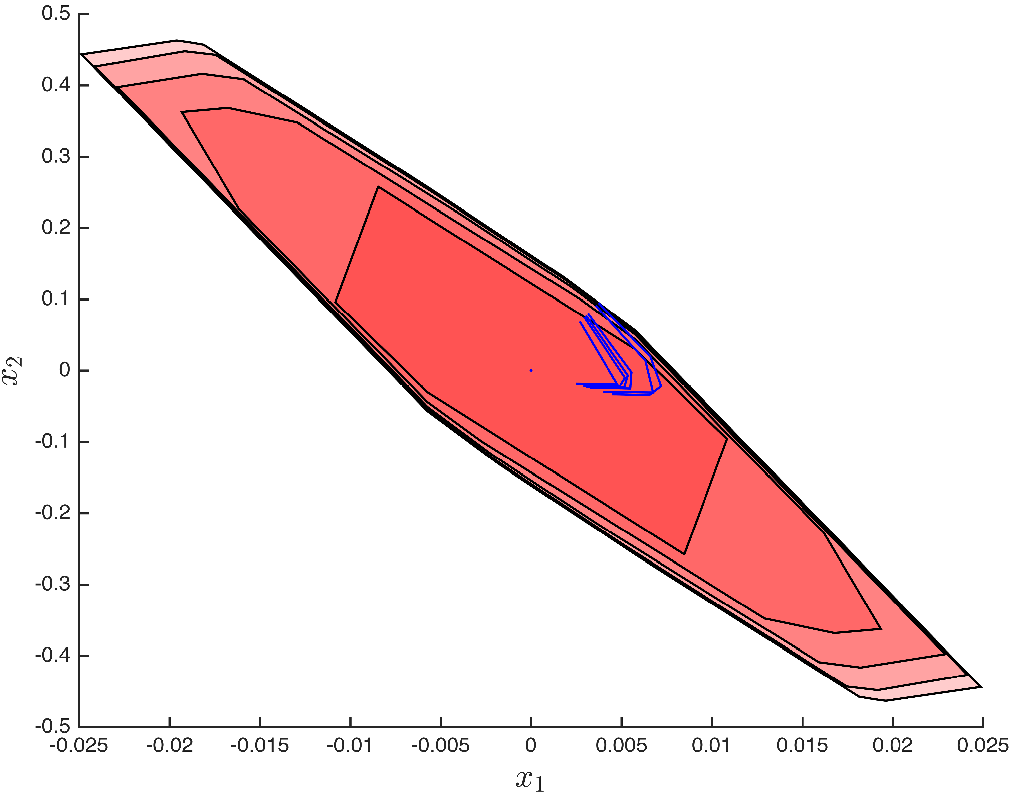
\includegraphics[width=\columnwidth]{myplot}
\caption{Projected stage constraints $\mathcal X_i$, $i\in\mathbb N_N$
% $i=1,\dots,N$ 
in red. Trajectories
at the active set changes and on the boundary in blue.}
\label{fig:plot}
\end{figure}

\begin{figure}
\centering
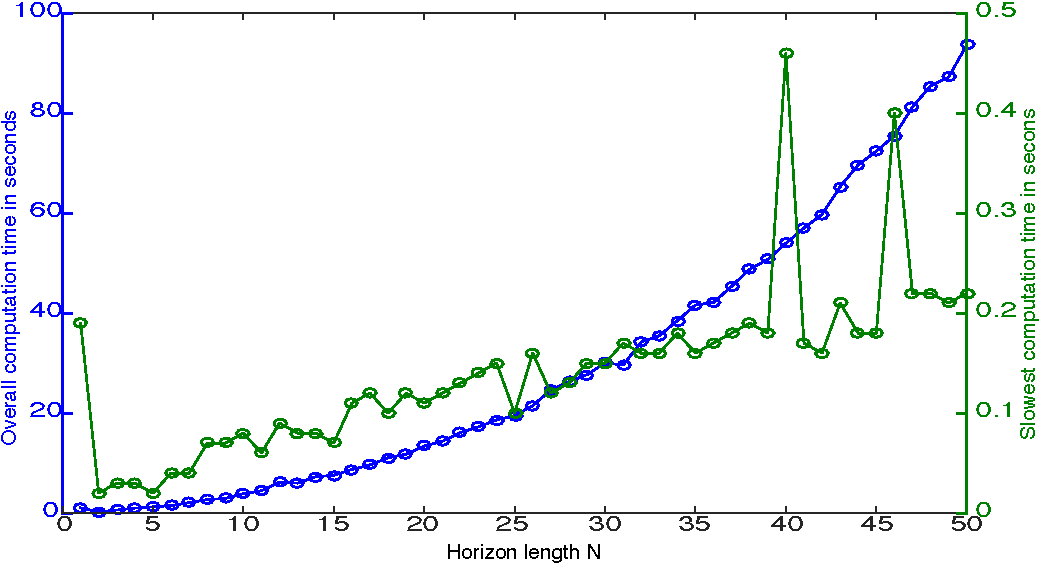
\includegraphics[width=\columnwidth]{ComputationTimes.pdf}
\caption{The \textcolor[rgb]{0,0,1}{blue points} show the overall computation time from a cold start 
at~$x_a=(0,0)$ to the boundary of the feasible set. The \textcolor[rgb]{0,.6,0}{green points} show the slowest recursion
performed which approximately is linear.}
\label{fig:computation:times}
\end{figure}


% needed in second column of first page if using \IEEEpubid
%\IEEEpubidadjcol


% An example of a floating figure using the graphicx package.
% Note that \label must occur AFTER (or within) \caption.
% For figures, \caption should occur after the \includegraphics.
% Note that IEEEtran v1.7 and later has special internal code that
% is designed to preserve the operation of \label within \caption
% even when the captionsoff option is in effect. However, because
% of issues like this, it may be the safest practice to put all your
% \label just after \caption rather than within \caption{}.
%
% Reminder: the "draftcls" or "draftclsnofoot", not "draft", class
% option should be used if it is desired that the figures are to be
% displayed while in draft mode.
%
%\begin{figure}[!t]
%\centering
%\includegraphics[width=2.5in]{myfigure}
% where an .eps filename suffix will be assumed under latex, 
% and a .pdf suffix will be assumed for pdflatex; or what has been declared
% via \DeclareGraphicsExtensions.
%\caption{Simulation results for the network.}
%\label{fig_sim}
%\end{figure}

% Note that IEEE typically puts floats only at the top, even when this
% results in a large percentage of a column being occupied by floats.


% An example of a double column floating figure using two subfigures.
% (The subfig.sty package must be loaded for this to work.)
% The subfigure \label commands are set within each subfloat command,
% and the \label for the overall figure must come after \caption.
% \hfil is used as a separator to get equal spacing.
% Watch out that the combined width of all the subfigures on a 
% line do not exceed the text width or a line break will occur.
%
%\begin{figure*}[!t]
%\centering
%\subfloat[Case I]{\includegraphics[width=2.5in]{box}%
%\label{fig_first_case}}
%\hfil
%\subfloat[Case II]{\includegraphics[width=2.5in]{box}%
%\label{fig_second_case}}
%\caption{Simulation results for the network.}
%\label{fig_sim}
%\end{figure*}
%
% Note that often IEEE papers with subfigures do not employ subfigure
% captions (using the optional argument to \subfloat[]), but instead will
% reference/describe all of them (a), (b), etc., within the main caption.
% Be aware that for subfig.sty to generate the (a), (b), etc., subfigure
% labels, the optional argument to \subfloat must be present. If a
% subcaption is not desired, just leave its contents blank,
% e.g., \subfloat[].


% An example of a floating table. Note that, for IEEE style tables, the
% \caption command should come BEFORE the table and, given that table
% captions serve much like titles, are usually capitalized except for words
% such as a, an, and, as, at, but, by, for, in, nor, of, on, or, the, to
% and up, which are usually not capitalized unless they are the first or
% last word of the caption. Table text will default to \footnotesize as
% IEEE normally uses this smaller font for tables.
% The \label must come after \caption as always.
%
%\begin{table}[!t]
%% increase table row spacing, adjust to taste
%\renewcommand{\arraystretch}{1.3}
% if using array.sty, it might be a good idea to tweak the value of
% \extrarowheight as needed to properly center the text within the cells
%\caption{An Example of a Table}
%\label{table_example}
%\centering
%% Some packages, such as MDW tools, offer better commands for making tables
%% than the plain LaTeX2e tabular which is used here.
%\begin{tabular}{|c||c|}
%\hline
%One & Two\\
%\hline
%Three & Four\\
%\hline
%\end{tabular}
%\end{table}


% Note that the IEEE does not put floats in the very first column
% - or typically anywhere on the first page for that matter. Also,
% in-text middle ("here") positioning is typically not used, but it
% is allowed and encouraged for Computer Society conferences (but
% not Computer Society journals). Most IEEE journals/conferences use
% top floats exclusively. 
% Note that, LaTeX2e, unlike IEEE journals/conferences, places
% footnotes above bottom floats. This can be corrected via the
% \fnbelowfloat command of the stfloats package.




\section{Conclusion}\label{sec:conclusion}
In this paper we present a framework to treat robust model predictive control problems that are formulated with state and input dependent disturbance constraints.
%
These problems are formulated as a sequence of min-max programs where the constraints at each stage are chosen in such a way that at the last stage the state is contained in the maximal positive robust invariant set.
%
In order to determine the MRPI set for a constrained system with state dependent disturbances a key property is \emph{parametric convexity}, which the disturbance set necessarily has to have in order to guarantee the convexity of the MRPI set.
%
For a polytopic setup in connection with parametric convexity of a piecewise affine disturbance set we prove the finite determinability of the MRPI set.
%
\par The quadratic min-max sequence is solved recursively by an active-set based approach. 
%
For a known sequence of active constraints the optimal control strategy is affine in the initial state, this optimal strategy is then updated with a line-search through the state space towards the current state when necessary.
%
Both main concepts are illustrated with a numerical example.
%
\par The complexity of the solver is linear in the horizon length for each set of active constraints, however in general no practically useful bound on the number of active-set updates can be given. 
%





% if have a single appendix:
%\appendix[Proof of the Zonklar Equations]
% or
%\appendix  % for no appendix heading
% do not use \section anymore after \appendix, only \section*
% is possibly needed

% use appendices with more than one appendix
% then use \section to start each appendix
% you must declare a \section before using any
% \subsection or using \label (\appendices by itself
% starts a section numbered zero.)
%


\appendices


% use section* for acknowledgment
\section*{Acknowledgment}

The first author is supported by the Worcester College Senior Scholarship and an EPSRC doctoral studentship.  

% \section*{Appendix}

% \textit{Proof of Proposition~\ref{prop:Dk:iteration}.}\hspace{1ex}%
% %
% Since $\mathcal{D}_k$ is the set of states for which the $k$ steps ahead state lies in $\mathcal{X}$, we have $\mathcal{D}_0 = \mathcal{X}$ and
% %, for $k\geq 1$,
% \[
% \mathcal{D}_k = \bigl\{ x : \{\Psi x\} \oplus \mathcal{V}(x) \subseteq \mathcal{D}_{k-1}\bigr\}  
% \ \forall k = 1,2\ldots 
% \]
% Hence for $k\geq 1$, $\Psi^k \mathcal{D}_k$ is given by
% \begin{align*}
% \Psi^k\mathcal{D}_k &= \bigl\{ \Psi^k x : \{\Psi x\} \oplus \mathcal{V}(x) \subseteq \mathcal{D}_{k-1}\bigr\} \\
% & = \bigl\{ y : \{\Psi^{-k+1} y\} \oplus \mathcal{V}_k(y) \subseteq \mathcal{D}_{k-1}\bigr\} \\
% & = \bigl\{ y : \{ y\} \oplus \Psi^{k-1}\mathcal{V}_k(y) \subseteq \Psi^{k-1}\mathcal{D}_{k-1}\bigr\} .
% \end{align*}
% Using the definition of the parametric Pontryagin difference, this implies
% \[
% \Psi^{k}\mathcal{D}_k = (\Psi^{k-1}\mathcal{D}_{k-1}) \ominus \Psi^{k-1}\mathcal{V}_k(\Psi^{k-1}\mathcal{D}_{k-1}) \ \forall k=1,2\ldots 
% \]
% and the result therefore follows from  $\mathcal{R}_0=\mathcal{D}_0$ and (\ref{eq:Rk:iteration}).%
% %
% % so if $\Psi^{k}\mathcal{D}_k = \mathcal{R}_k$ and $\Psi^{k-1}\mathcal{D}_{k-1} = \mathcal{R}_{k-1}$, then by the definition of the parametric Pontryagin difference we have
% % \[
% % \mathcal{R}_k = \mathcal{R}_{k-1}\ominus \Psi^{k-1} \mathcal{V}_k(\mathcal{R}_{k-1}), \ \forall k=1,2,\ldots,
% % \]
% % and the result follows from
% % (\ref{eq:Rk:iteration}) and $\mathcal{R}_0=\mathcal{D}_0 = \mathcal{X}$.
% %\end{proof}%
% \hfill\qed


% Can use something like this to put references on a page
% by themselves when using endfloat and the captionsoff option.
\ifCLASSOPTIONcaptionsoff
  \newpage
\fi



% trigger a \newpage just before the given reference
% number - used to balance the columns on the last page
% adjust value as needed - may need to be readjusted if
% the document is modified later
%\IEEEtriggeratref{8}
% The "triggered" command can be changed if desired:
%\IEEEtriggercmd{\enlargethispage{-5in}}

% references section

% can use a bibliography generated by BibTeX as a .bbl file
% BibTeX documentation can be easily obtained at:
% http://www.ctan.org/tex-archive/biblio/bibtex/contrib/doc/
% The IEEEtran BibTeX style support page is at:
% http://www.michaelshell.org/tex/ieeetran/bibtex/
\bibliographystyle{IEEEtran}
% argument is your BibTeX string definitions and bibliography database(s)
\bibliography{IEEEabrv,MyLib}

%
% <OR> manually copy in the resultant .bbl file
% set second argument of \begin to the number of references
% (used to reserve space for the reference number labels box)
% \begin{thebibliography}{1}

% \end{thebibliography}

% biography section
% 
% If you have an EPS/PDF photo (graphicx package needed) extra braces are
% needed around the contents of the optional argument to biography to prevent
% the LaTeX parser from getting confused when it sees the complicated
% \includegraphics command within an optional argument. (You could create
% your own custom macro containing the \includegraphics command to make things
% simpler here.)
%\begin{IEEEbiography}[{\includegraphics[width=1in,height=1.25in,clip,keepaspectratio]{mshell}}]{Michael Shell}
% or if you just want to reserve a space for a photo:

\begin{IEEEbiography}[{
\includegraphics[width=1in,height=1.25in,clip,keepaspectratio]{face.pdf}}]{Rainer Manuel Schaich}
Biography text here.
\end{IEEEbiography}

% if you will not have a photo at all:
\begin{IEEEbiography}[{
\includegraphics[width=1in,height=1.25in,clip,keepaspectratio]{face.pdf}}]{Mark Cannon}
Biography text here.
\end{IEEEbiography}

% insert where needed to balance the two columns on the last page with
% biographies
%\newpage

% You can push biographies down or up by placing
% a \vfill before or after them. The appropriate
% use of \vfill depends on what kind of text is
% on the last page and whether or not the columns
% are being equalized.

%\vfill

% Can be used to pull up biographies so that the bottom of the last one
% is flush with the other column.
%\enlargethispage{-5in}



% that's all folks
\end{document}


